% !TEX root = ./supplementary.tex
%  Supplementary Materials — Chill branch
%=================================================================
\documentclass[agriengineering,supfile,submit,pdftex,moreauthors]{Definitions/mdpi}

\usepackage{siunitx}
\usepackage{booktabs}
\usepackage{changepage}
\usepackage{float}
\usepackage{placeins}

%=================================================================
\firstpage{1}
\makeatletter
\setcounter{page}{\@firstpage}
\makeatother
\pubvolume{1}
\issuenum{1}
\articlenumber{0}
\pubyear{2026}
\copyrightyear{2026}
\datereceived{ }
\daterevised{ }
\dateaccepted{ }
\datepublished{ }
\hreflink{https://doi.org/}

\graphicspath{
  {figures_final/}
}

%=================================================================
\Title{Chill-Window Attribution of ENSO-Driven Olive Yield Collapse on the Hyper-Arid Peruvian Coast}


\newcommand{\orcidauthorA}{0000-0002-5283-7211} % J. Quille-Mamani
\newcommand{\orcidauthorB}{0009-0003-8511-4524} % J. Huanuqueño-Murillo
\newcommand{\orcidauthorC}{0000-0003-3325-5512} % D. Quispe-Tito
\newcommand{\orcidauthorD}{0000-0002-4518-1023} % G. Huayna-Felipe
\newcommand{\orcidauthorE}{0000-0003-2236-8335} % J. Espinoza-Molina
\newcommand{\orcidauthorF}{0000-0003-1872-9062} % K. Acosta-Caipa
\newcommand{\orcidauthorG}{0009-0003-8329-6555} % H. S. Pérez-Cubas
\newcommand{\orcidauthorH}{0000-0002-0421-399X} % E. Ingol-Blanco
\newcommand{\orcidauthorI}{0000-0003-3946-7188} % L. Ramos-Fernández
\newcommand{\orcidauthorJ}{0000-0001-7432-4364} % E. Pino-Vargas

\Author{Javier Quille-Mamani $^{1}$\orcidA{},
Jos\'{e} Huanuque\~{n}o-Murillo $^{2}$\orcidB{},
David Quispe-Tito $^{2}$\orcidC{},
German Huayna-Felipe $^{3}$\orcidD{},
Jorge Espinoza-Molina $^{4}$\orcidE{},
Karina Acosta-Caipa $^{4}$\orcidF{},
Heler Samir P\'{e}rez-Cubas $^{5}$\orcidG{},
Eusebio Ingol-Blanco $^{6}$\orcidH{},
Lia Ramos-Fern\'{a}ndez $^{2,}$*\orcidI{} and
Edwin Pino-Vargas $^{7,}$*\orcidJ{}}

\AuthorNames{Javier Quille-Mamani, Jos\'{e} Huanuque\~{n}o-Murillo, David Quispe-Tito, German Huayna-Felipe, Jorge Espinoza-Molina, Karina Acosta-Caipa, Heler Samir P\'{e}rez-Cubas, Eusebio Ingol-Blanco, Lia Ramos-Fern\'{a}ndez, Edwin Pino-Vargas}
\AuthorCitation{Quille-Mamani, J.; Huanuque\~{n}o-Murillo, J.; Quispe-Tito, D.; Huayna-Felipe, G.; Espinoza-Molina, J.; Acosta-Caipa, K.; P\'{e}rez-Cubas, H.S.; Ingol-Blanco, E.; Ramos-Fern\'{a}ndez, L.; Pino-Vargas, E.}

\address{%
$^{1}$ \quad Geo-Environmental Cartography and Remote Sensing Group (CGAT), Universitat Polit\`{e}cnica de Val\`{e}ncia, Cam\'{i} de Vera s/n, 46022 Valencia, Spain\\
$^{2}$ \quad Department of Water Resources, National Agrarian University La Molina, Lima 15024, Peru\\
$^{3}$ \quad Master's Program in Water Resources, Jorge Basadre Grohmann National University, Tacna 23000, Peru\\
$^{4}$ \quad Department of Architecture, Jorge Basadre Grohmann National University, Tacna 23000, Peru\\
$^{5}$ \quad Department of Hydraulic Engineering and Environment, Universitat Polit\`{e}cnica de Val\`{e}ncia, Cam\'{i} de Vera s/n, 46022 Valencia, Spain\\
$^{6}$ \quad Department of Civil Engineering, New Mexico State University, Las Cruces, NM 88003, USA\\
$^{7}$ \quad Department of Civil Engineering, Jorge Basadre Grohmann National University, Tacna 23000, Peru}

\corres{Correspondence: liarf@lamolina.edu.pe (L.R.-F.); epinov@unjbg.edu.pe (E.P.-V.)}

\abstract{}
\keyword{}

%=================================================================
\begin{document}

\renewcommand{\thefigure}{S\arabic{figure}}
\renewcommand{\thetable}{S\arabic{table}}
\setcounter{figure}{0}
\setcounter{table}{0}

\section*{Supplementary Figures}

% -- Figure S1: Chill model comparison --
\begin{figure}[H]
\centering
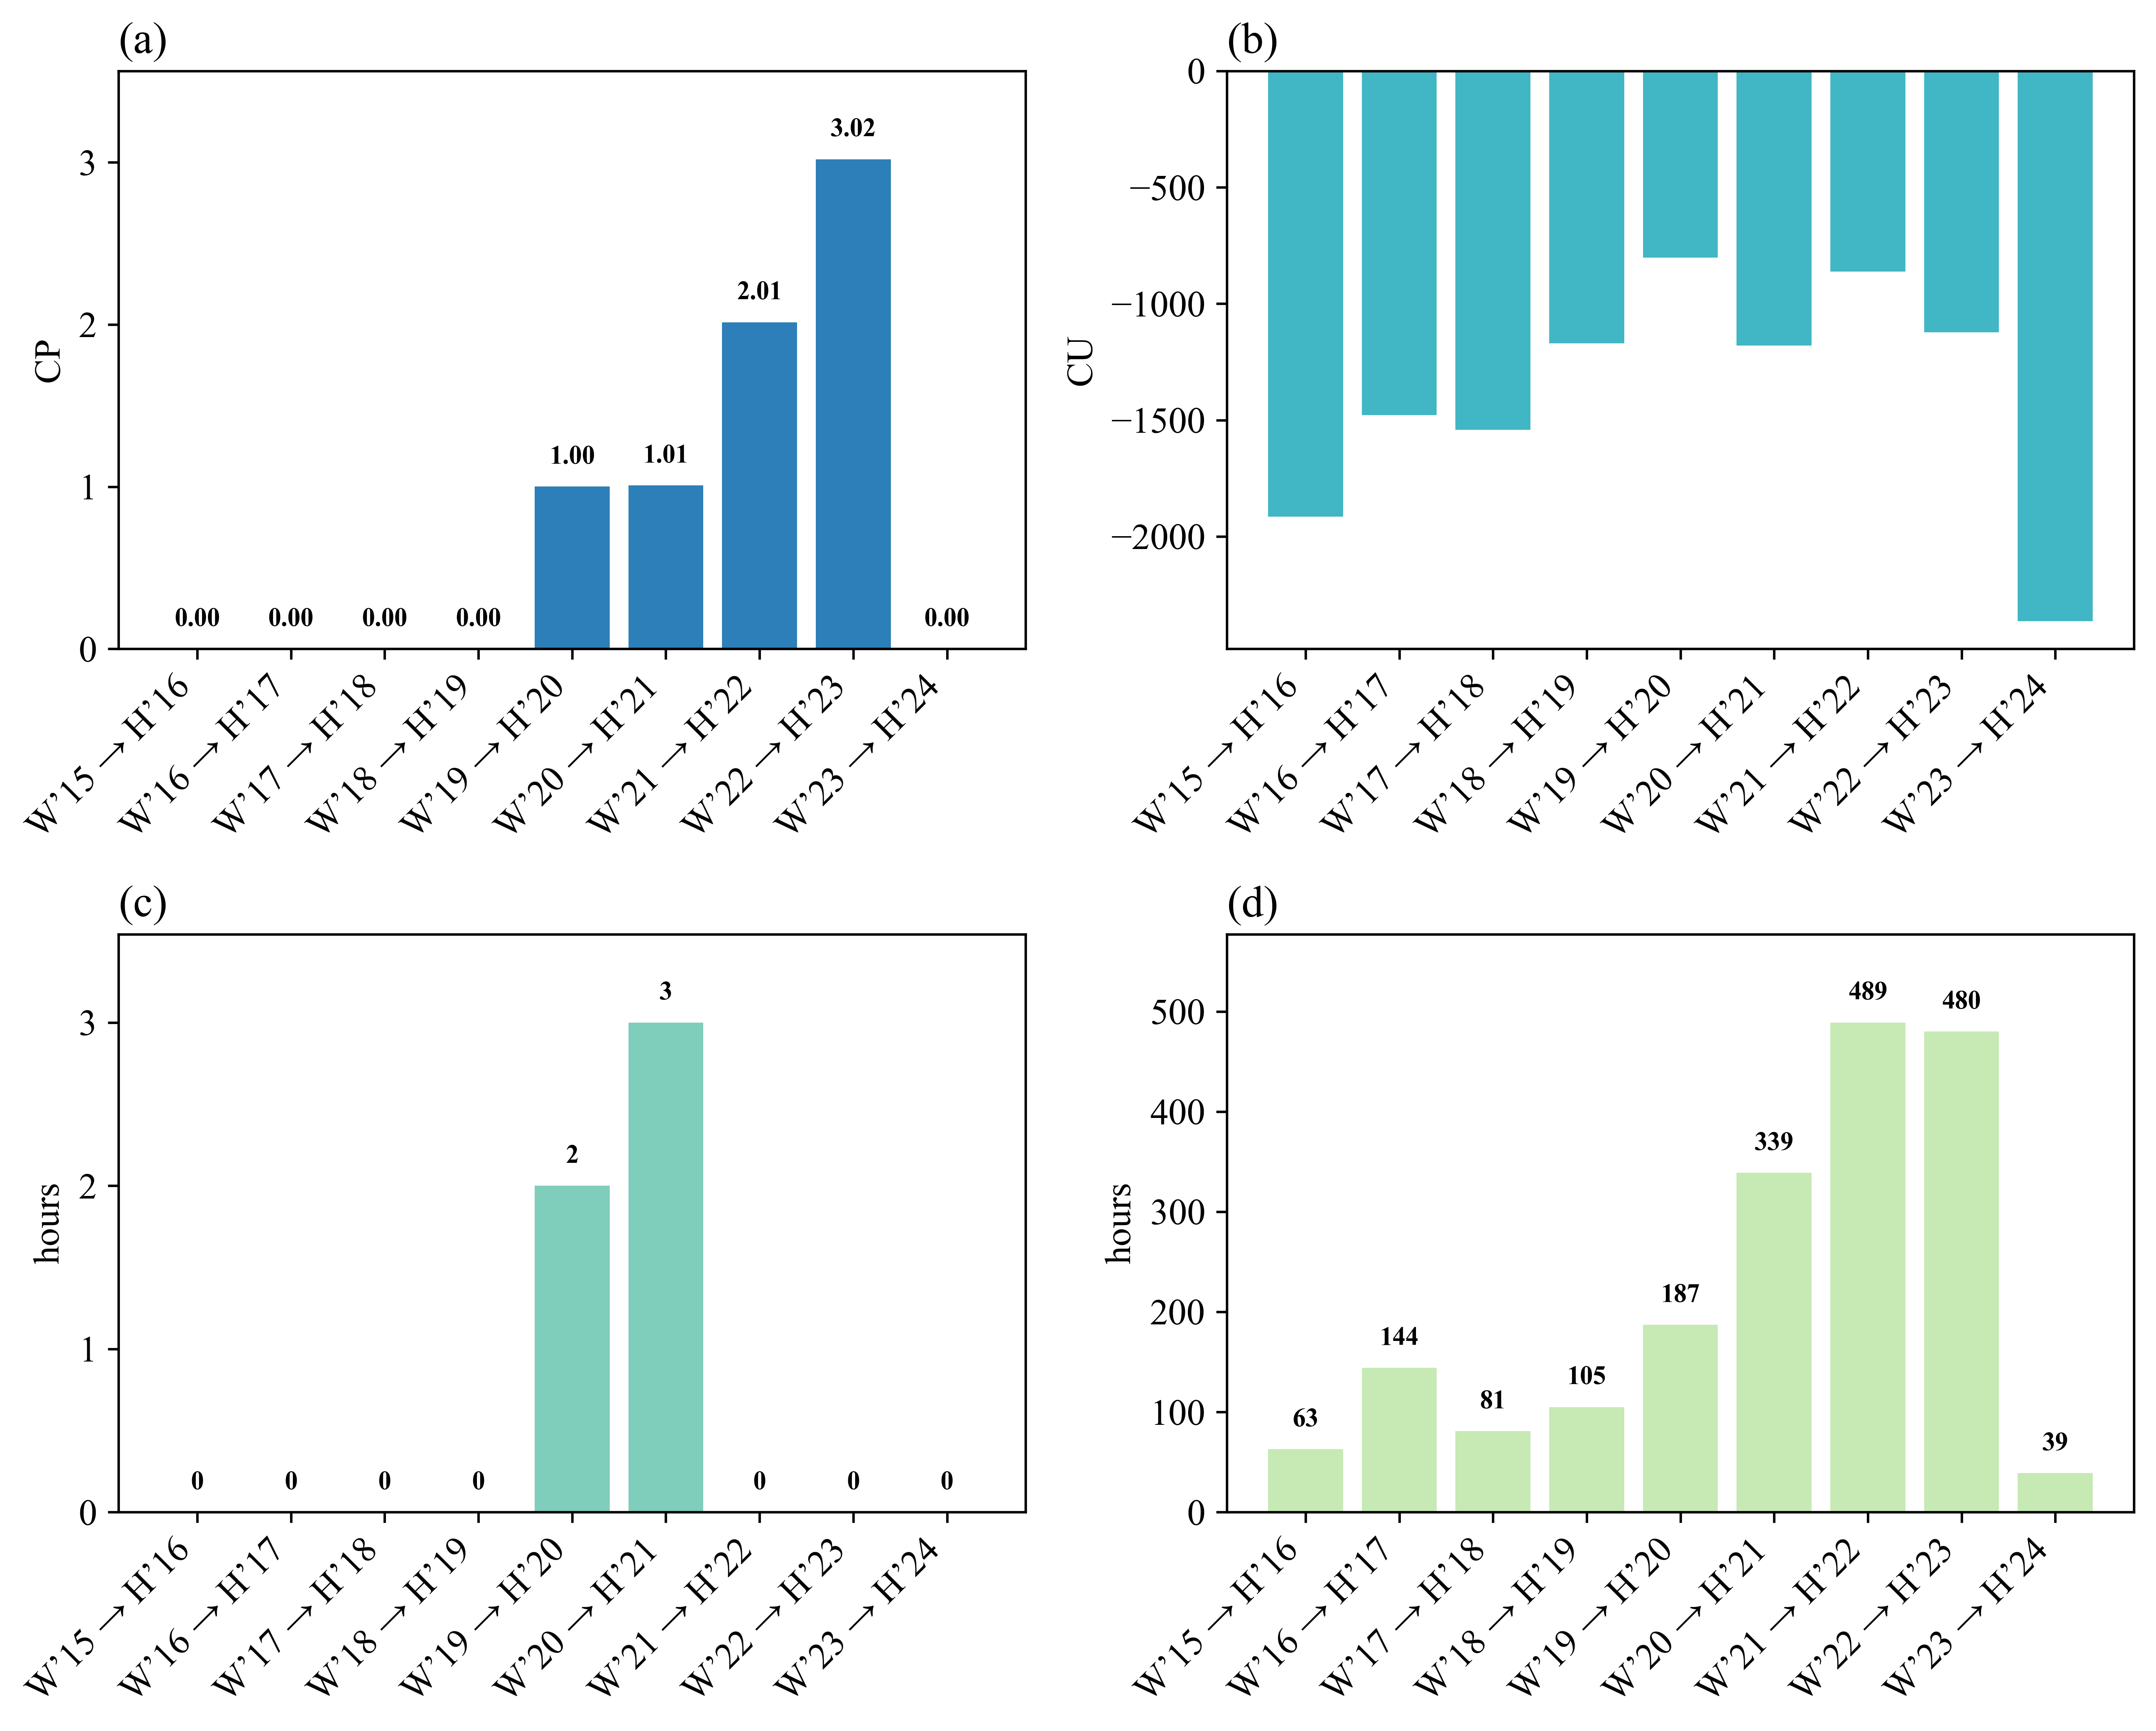
\includegraphics[width=\textwidth]{FigureS1.png}
\caption{Inter-comparison of chill-accumulation metrics over the May--August chill
window ($Y-1$) for the 2016--2024 study period. (\textbf{a})~Dynamic-Model Chill
Portions (CP); (\textbf{b})~Utah Chill Units (CU); (\textbf{c})~hours below
$7.2\,^{\circ}$C; (\textbf{d})~hours below $12\,^{\circ}$C. Bars are labelled
``W$'$YY $\to$ H$'$YY+1'' (chill winter $\to$ harvest year). CP floors at zero in
five of eight years, motivating the use of the chill-window mean temperature
$T_{\text{chill},t-1}$ as the primary chill predictor.\label{fig:S1}}
\end{figure}

% -- Figure S2: Partial chill effect --
\begin{figure}[H]
\centering
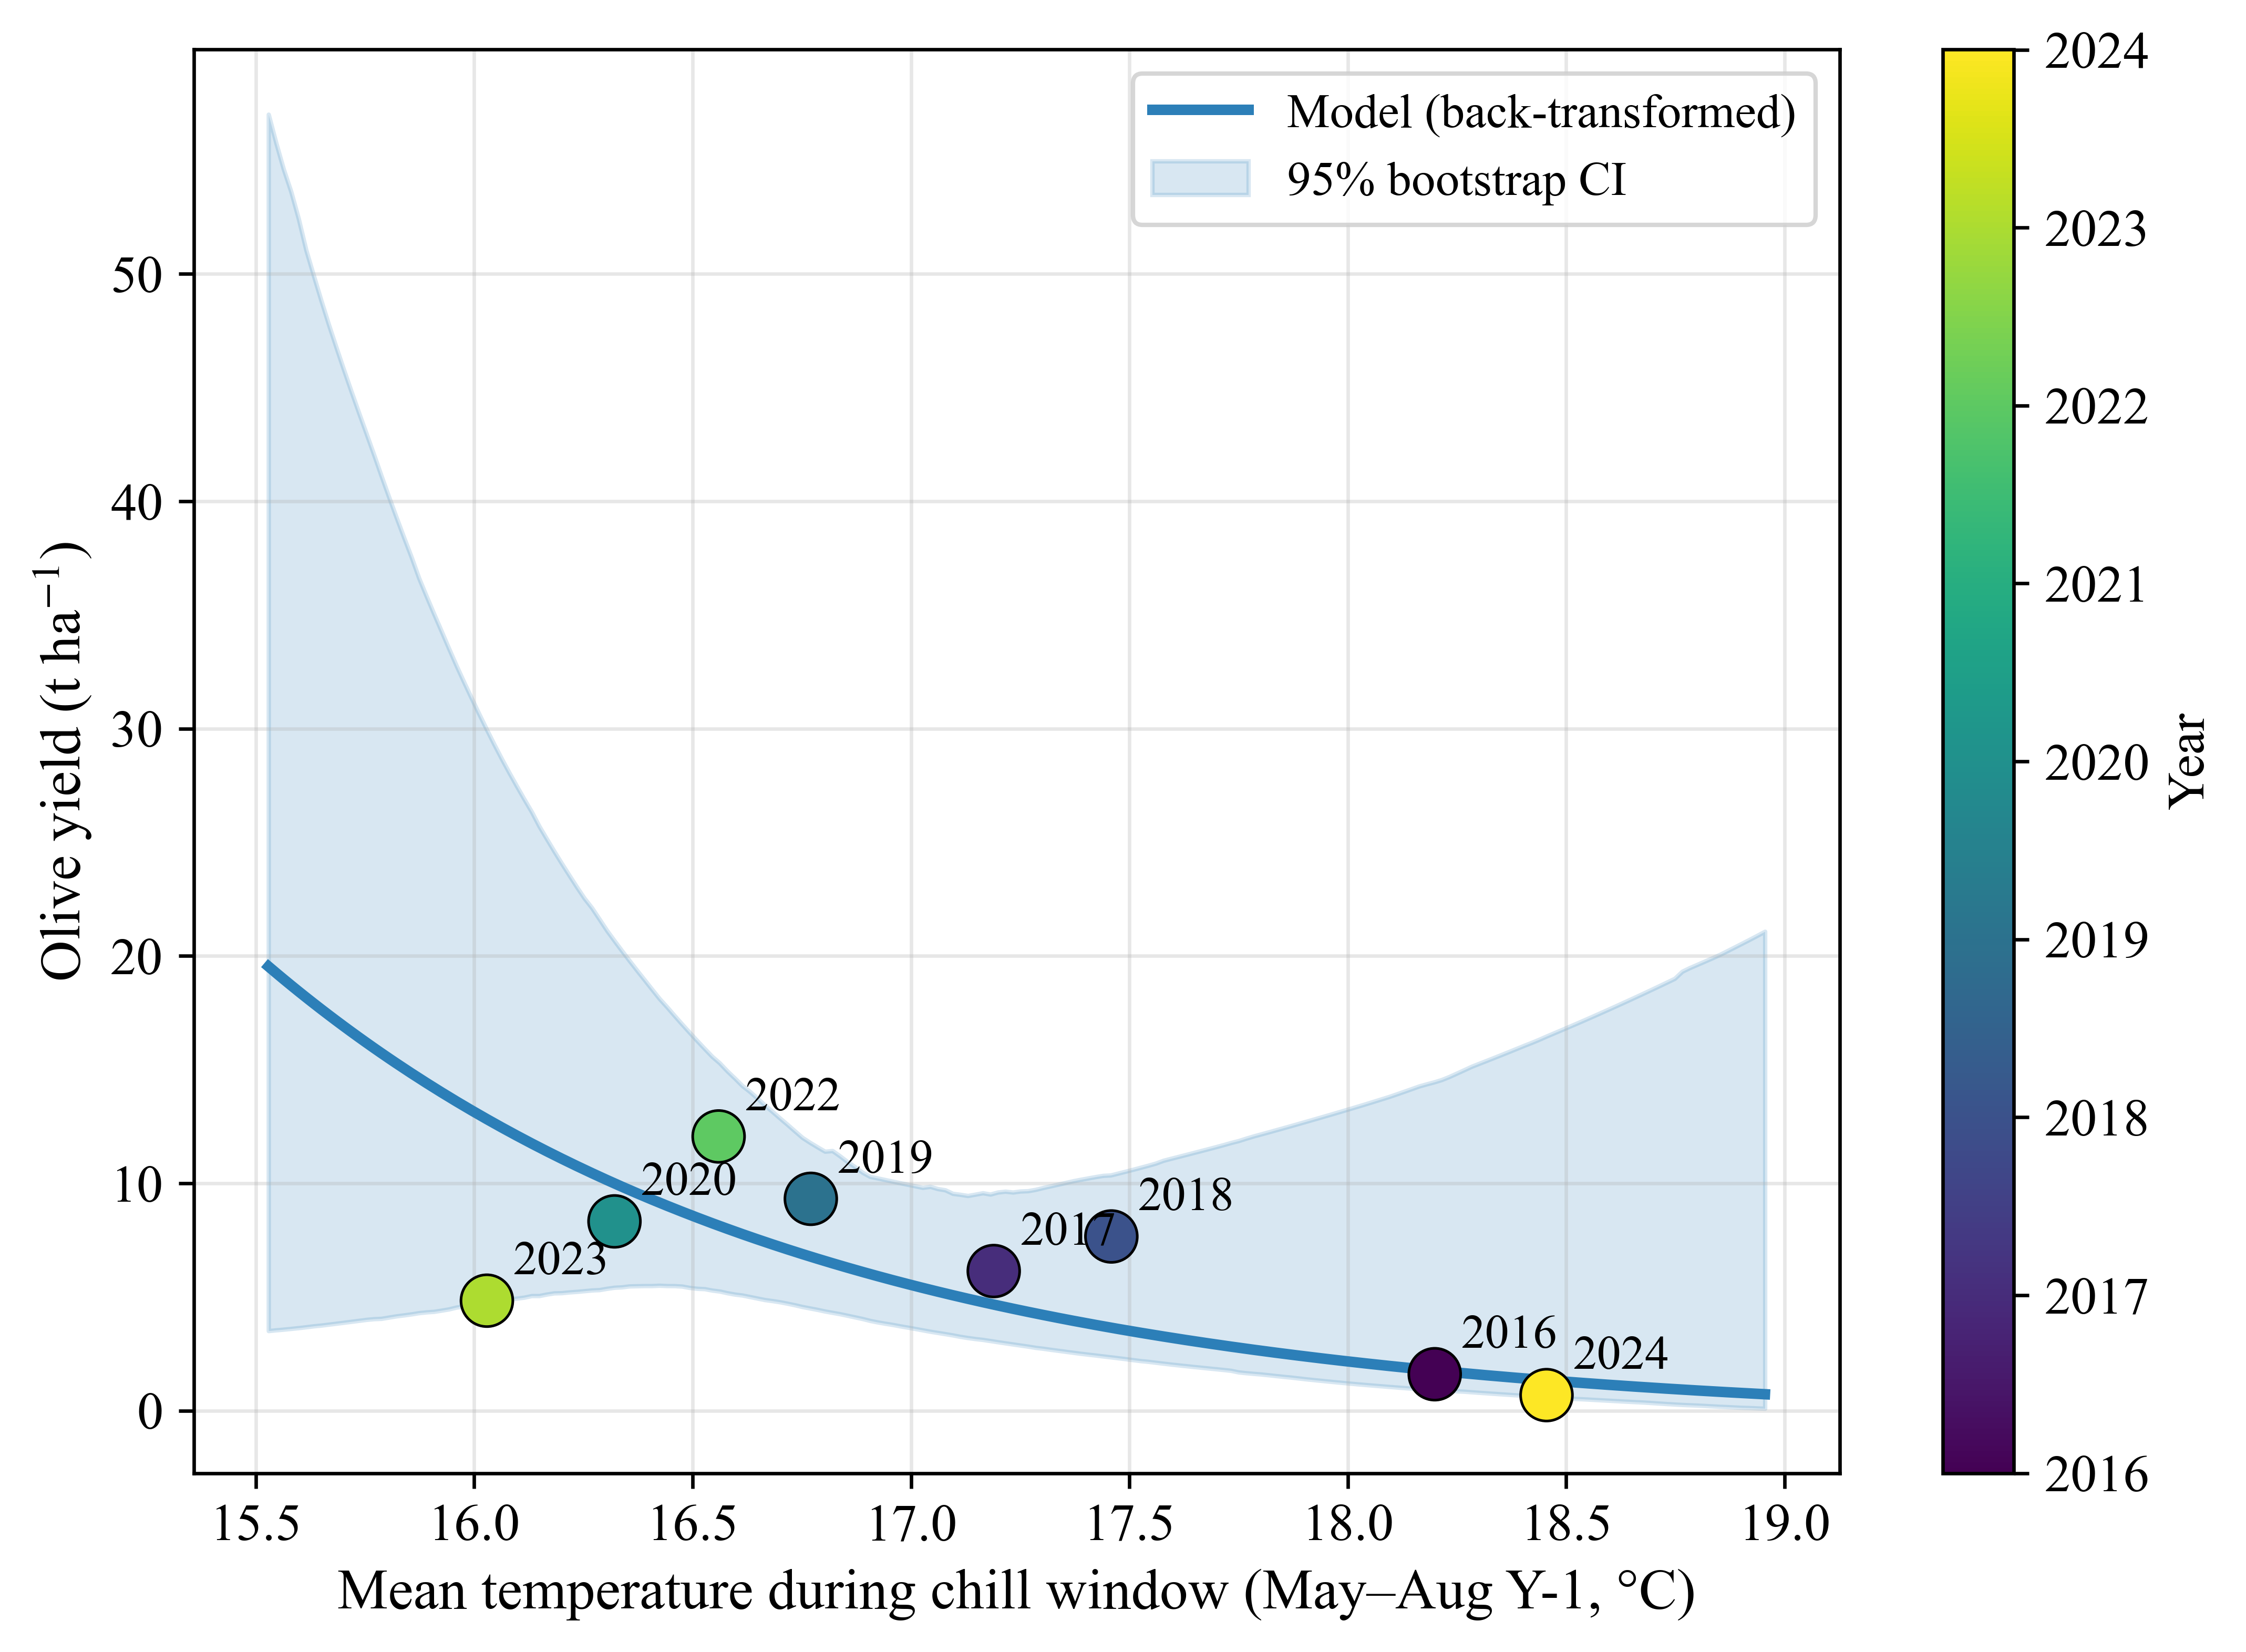
\includegraphics[width=0.85\textwidth]{FigureS2.png}
\caption{Partial-effect plot of $T_{\text{chill},t-1}$ on back-transformed olive
yield (t~ha$^{-1}$), holding $T_{\text{CREC},t}$ at its observed mean. Solid line:
primary log-OLS prediction back-transformed to the raw t~ha$^{-1}$ scale; shaded
band: year-block bootstrap 95\,\% CI ($B=5{,}000$). Points are observed yields
colour-coded by harvest year. The negative log-space slope
($\beta_{\text{chill}}=-0.816$, $p=0.030$) translates into the convex curve shown
here.\label{fig:S2}}
\end{figure}

% -- Figure S3: SSP yield bar chart --
\begin{figure}[H]
\centering
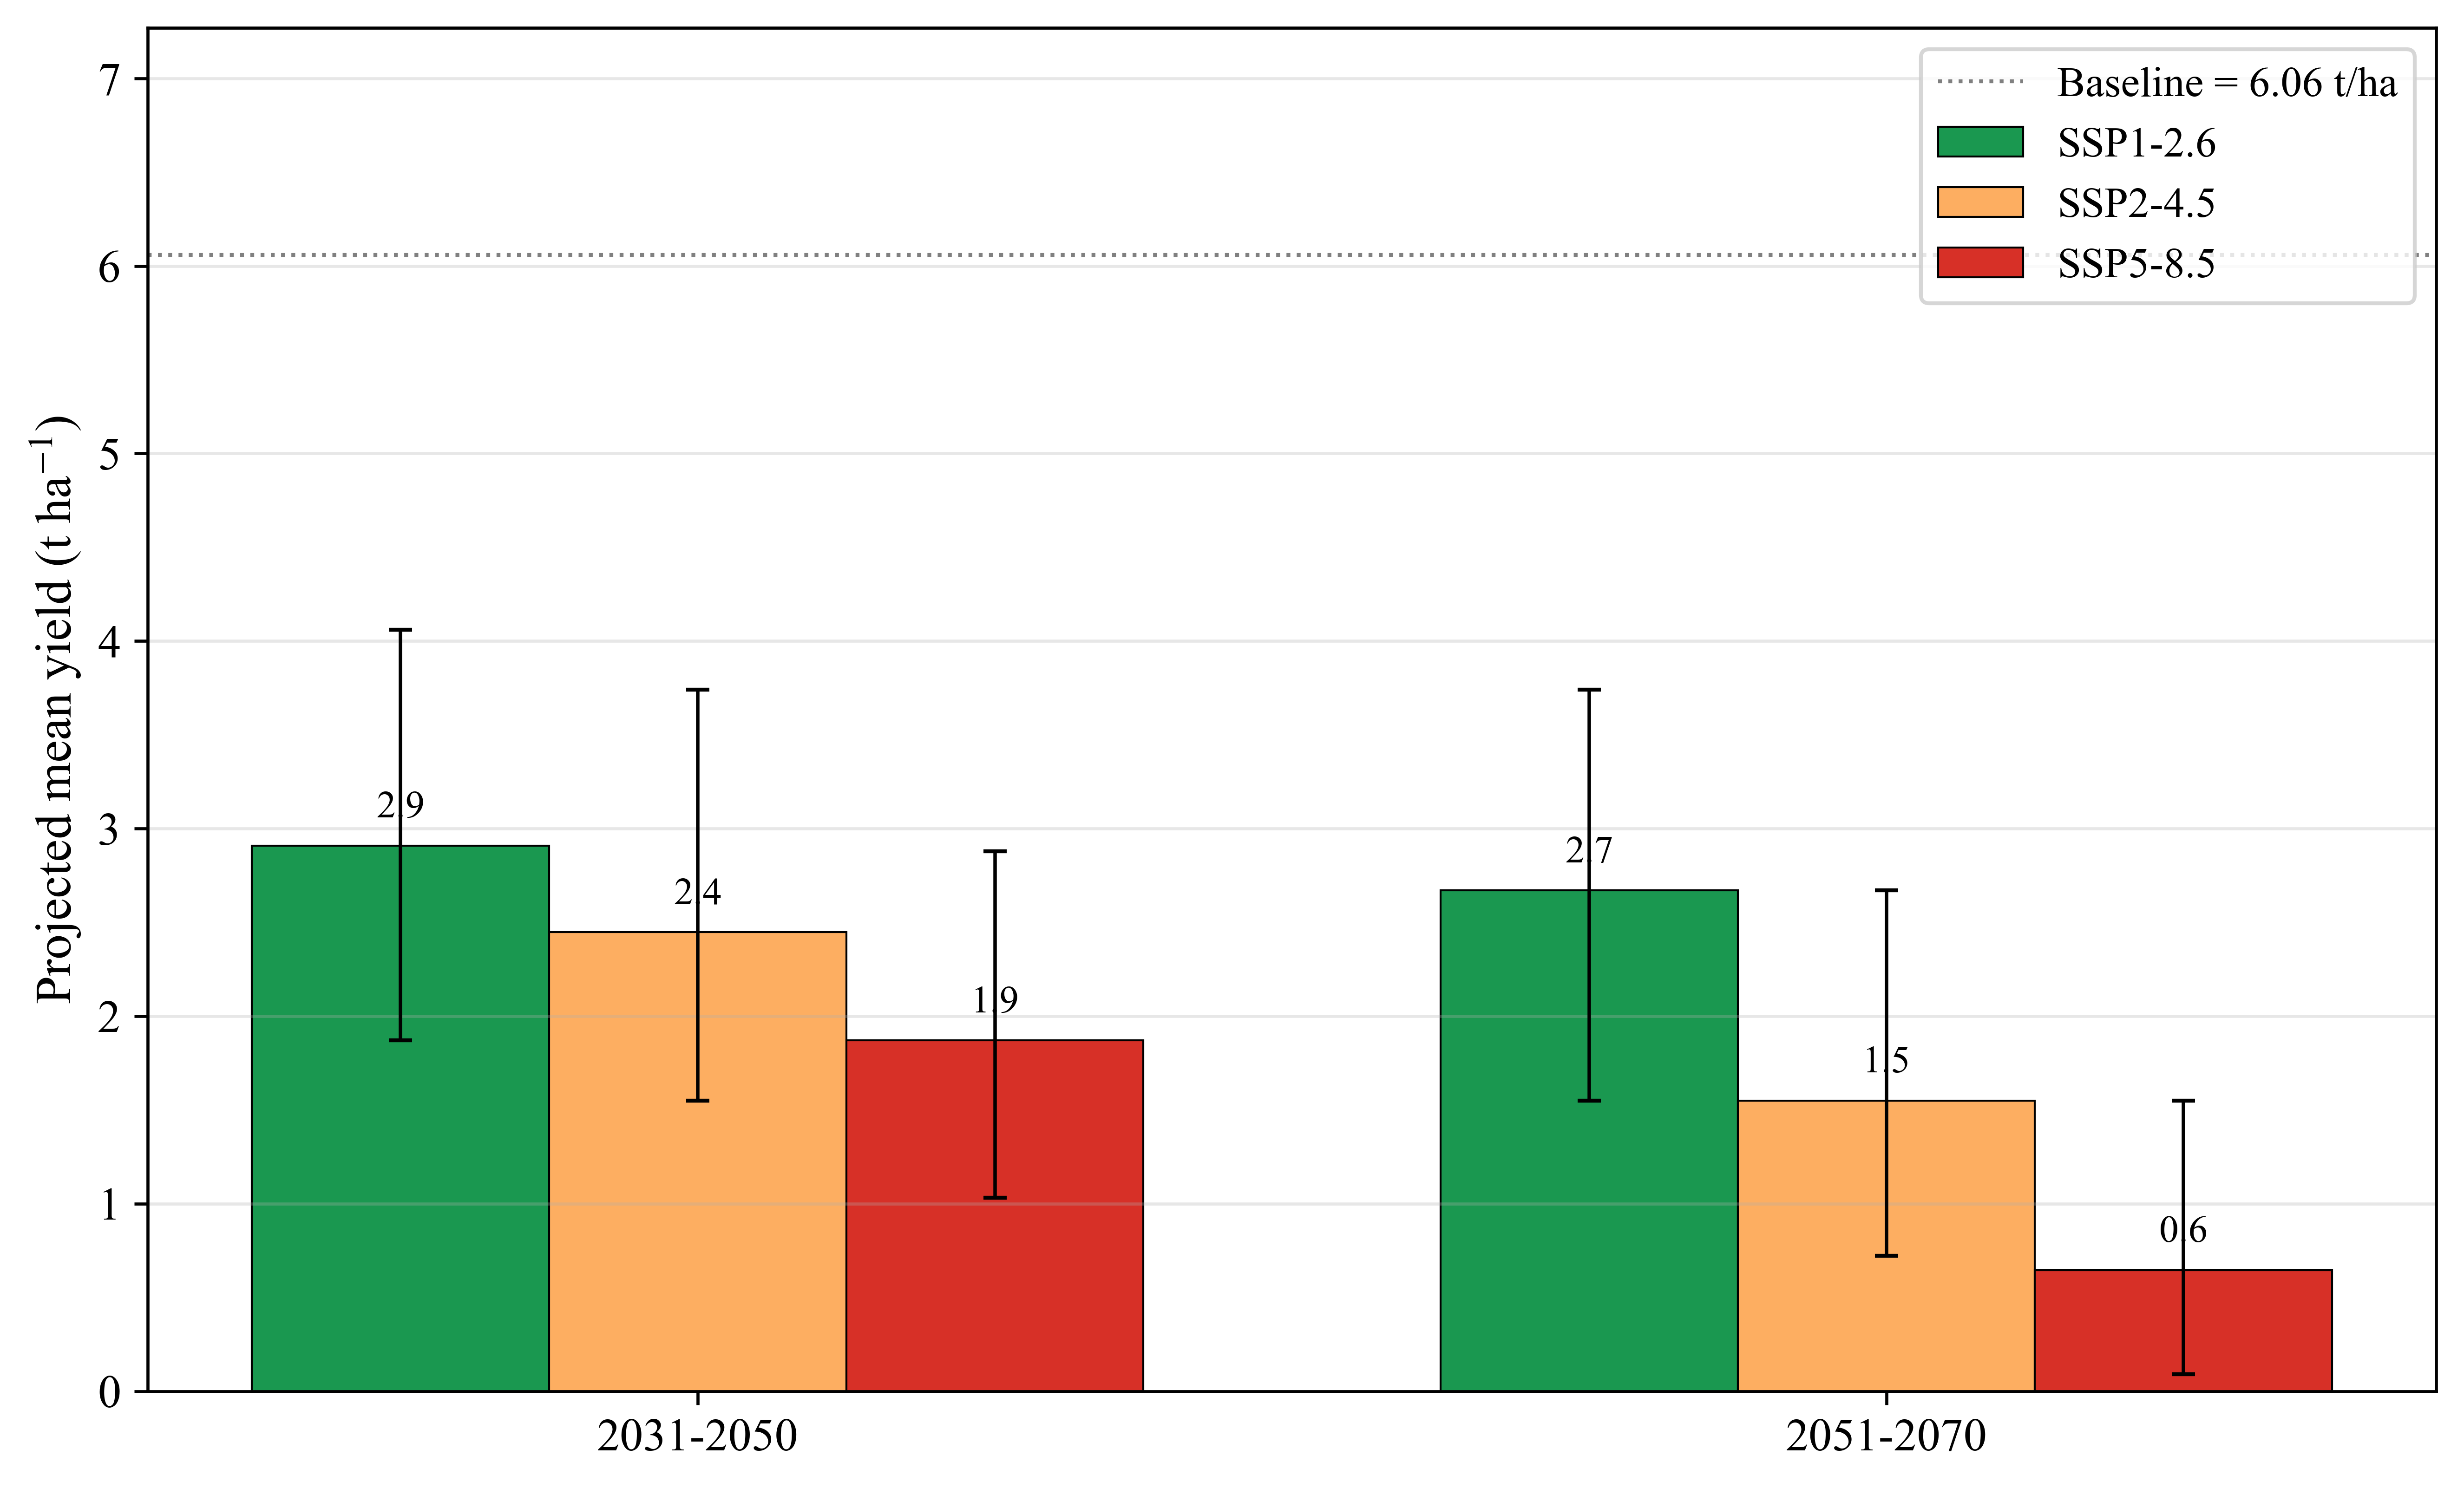
\includegraphics[width=\textwidth]{FigureS3.png}
\caption{CMIP6 delta-method projections of mean olive yield under three SSP
pathways (SSP1-2.6, SSP2-4.5, SSP5-8.5) and two time horizons (2031--2050,
2051--2070), relative to the calibrated baseline yield
($\bar y_0 = 6.06$~t~ha$^{-1}$; dashed line). Bars are central estimates obtained
with the IPCC AR6 WGI Atlas median warming for region SWS; whiskers span the
5--95\,\% inter-model envelope (Supplementary Table~\ref{tab:delta_envelope}).
Horizons beyond 2070 are omitted as extrapolative.\label{fig:S3}}
\end{figure}

% -- Figure S4: Chill collapse curve --
\begin{figure}[H]
\centering
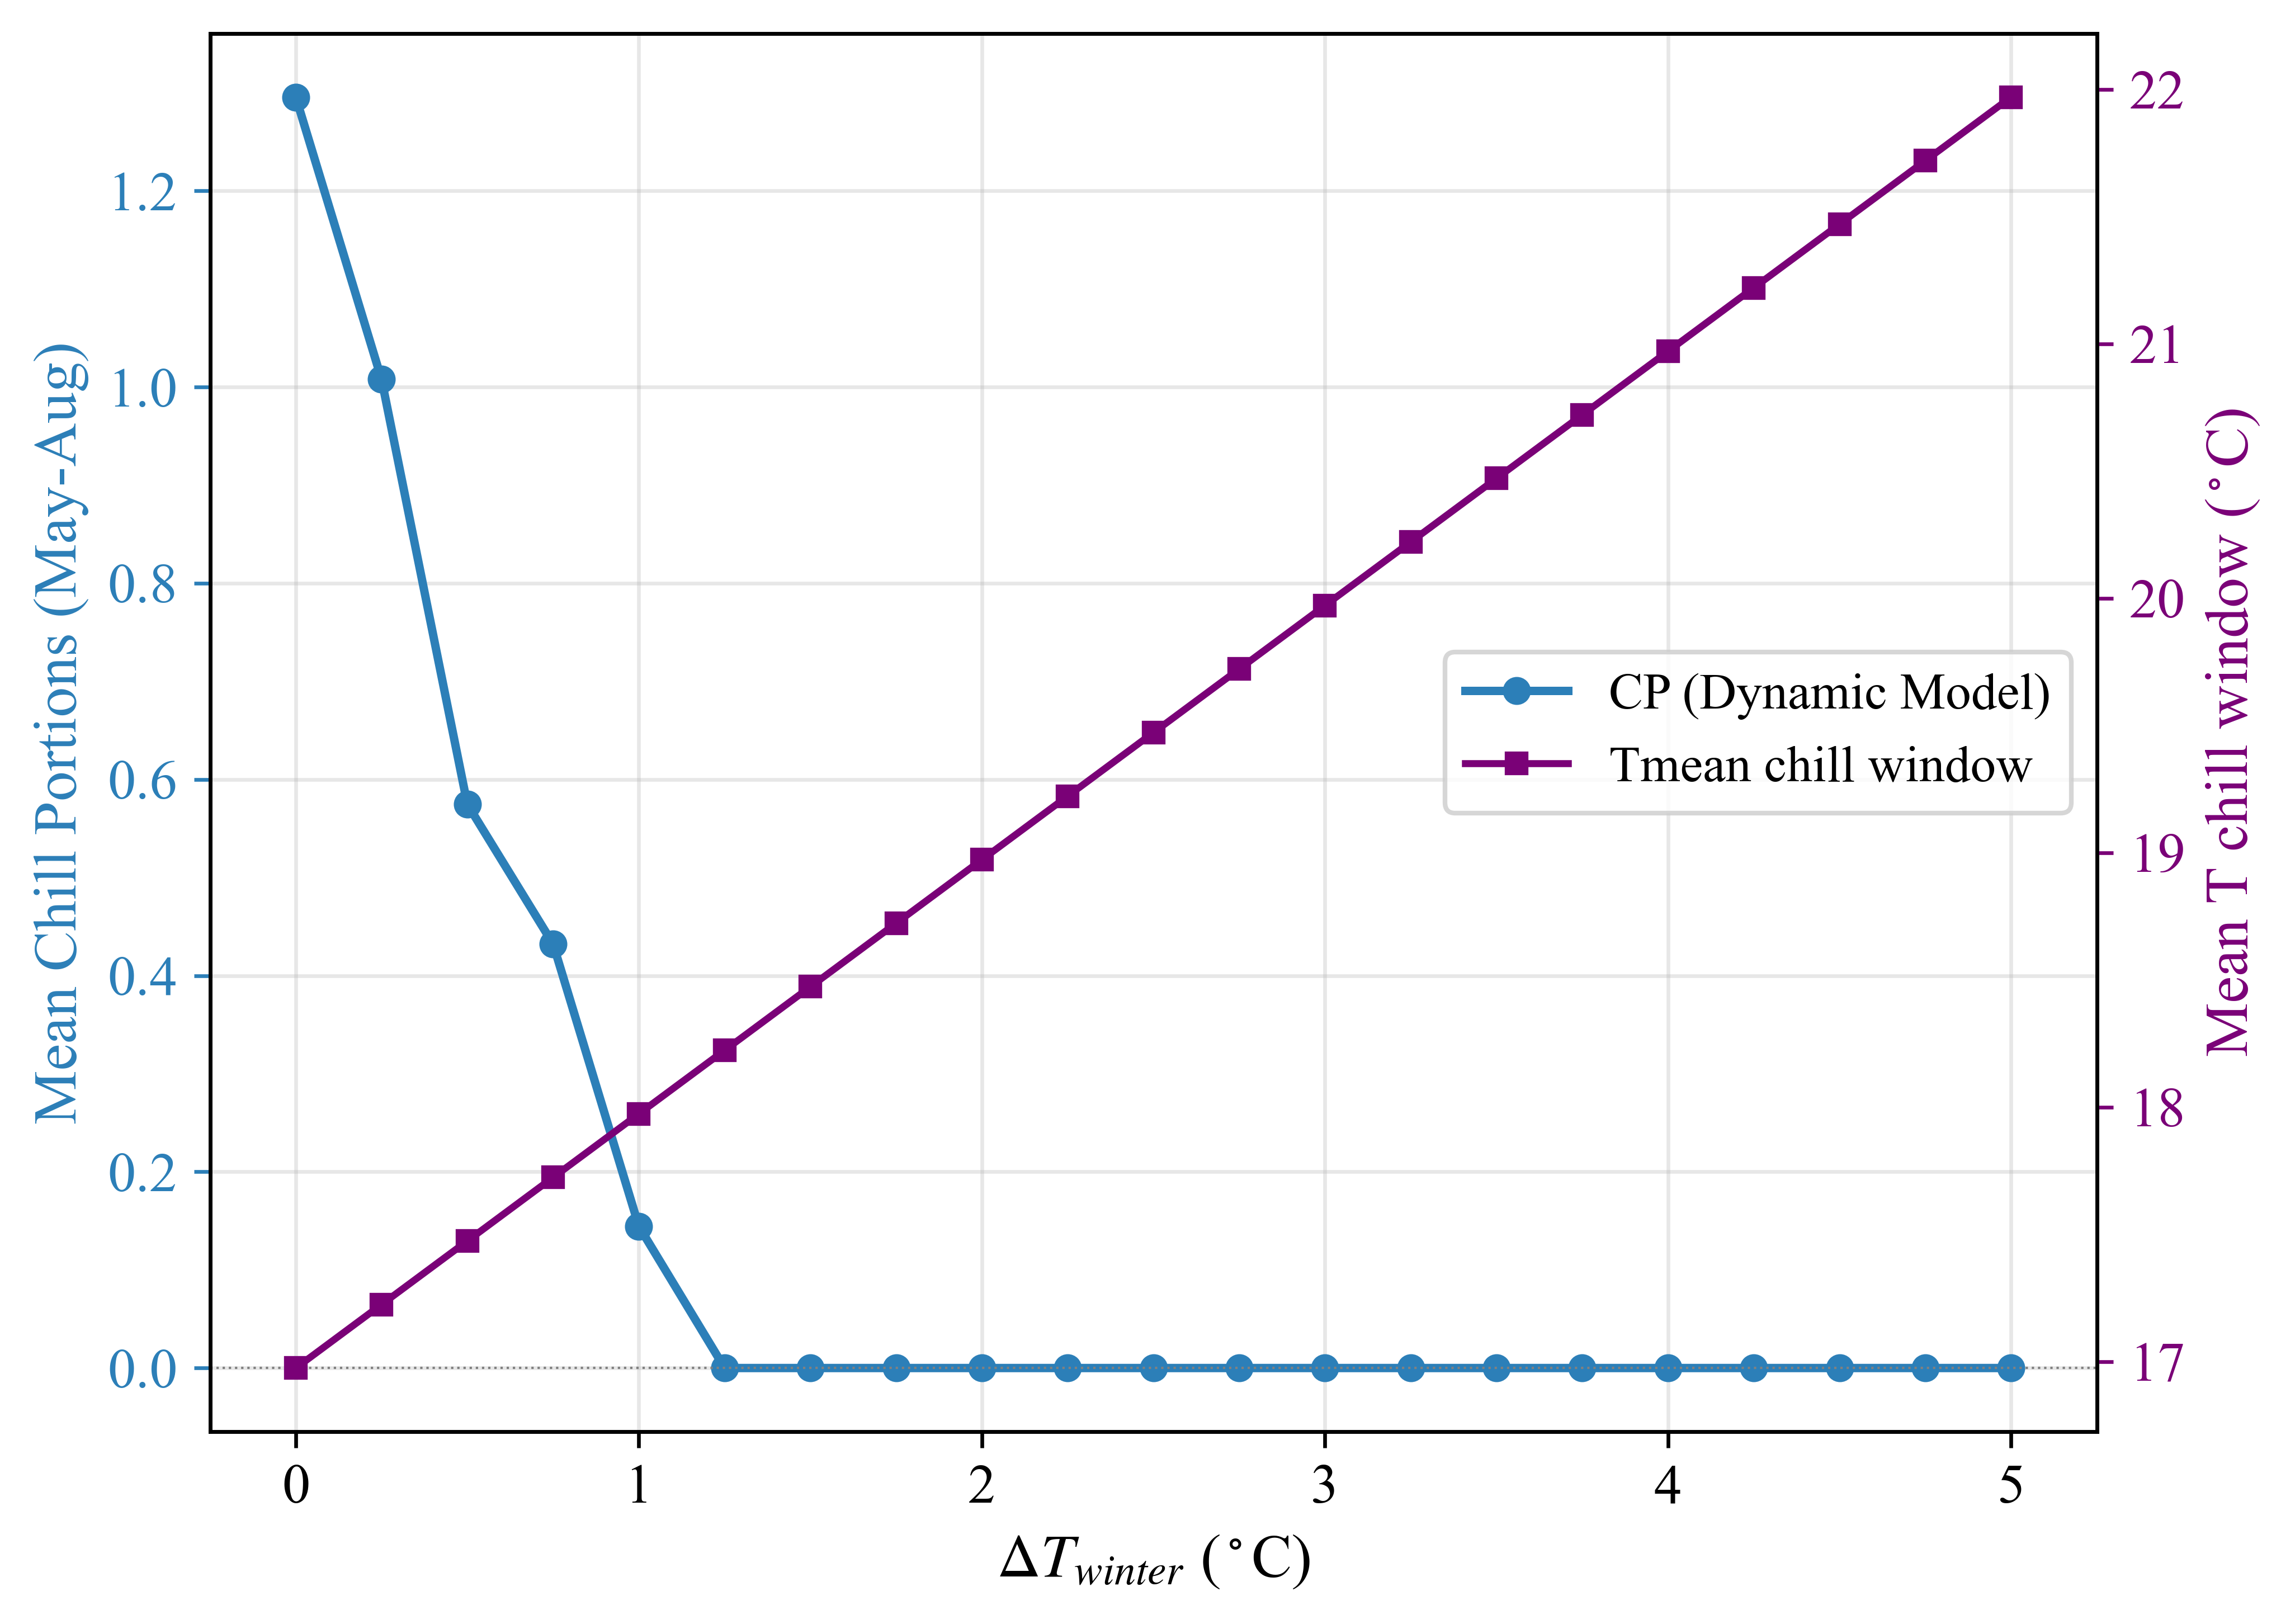
\includegraphics[width=0.9\textwidth]{FigureS4.png}
\caption{Chill-collapse mechanism: Dynamic-Model Chill Portions (CP, left axis,
blue) and chill-window mean temperature $T_{\text{chill}}$ (right axis, purple)
as functions of a uniform winter warming $\Delta T_{\text{winter}}$ applied to
the 2015--2025 chill-window daily series. CP collapses to zero at
$\Delta T_{\text{winter}}\approx +1.25\,^{\circ}$C, whereas $T_{\text{chill}}$
rises continuously, motivating $T_{\text{chill}}$ as the chill predictor in the
warm tail.\label{fig:S4}}
\end{figure}

% -- Figure S5: Residual diagnostics --
\begin{figure}[H]
\centering
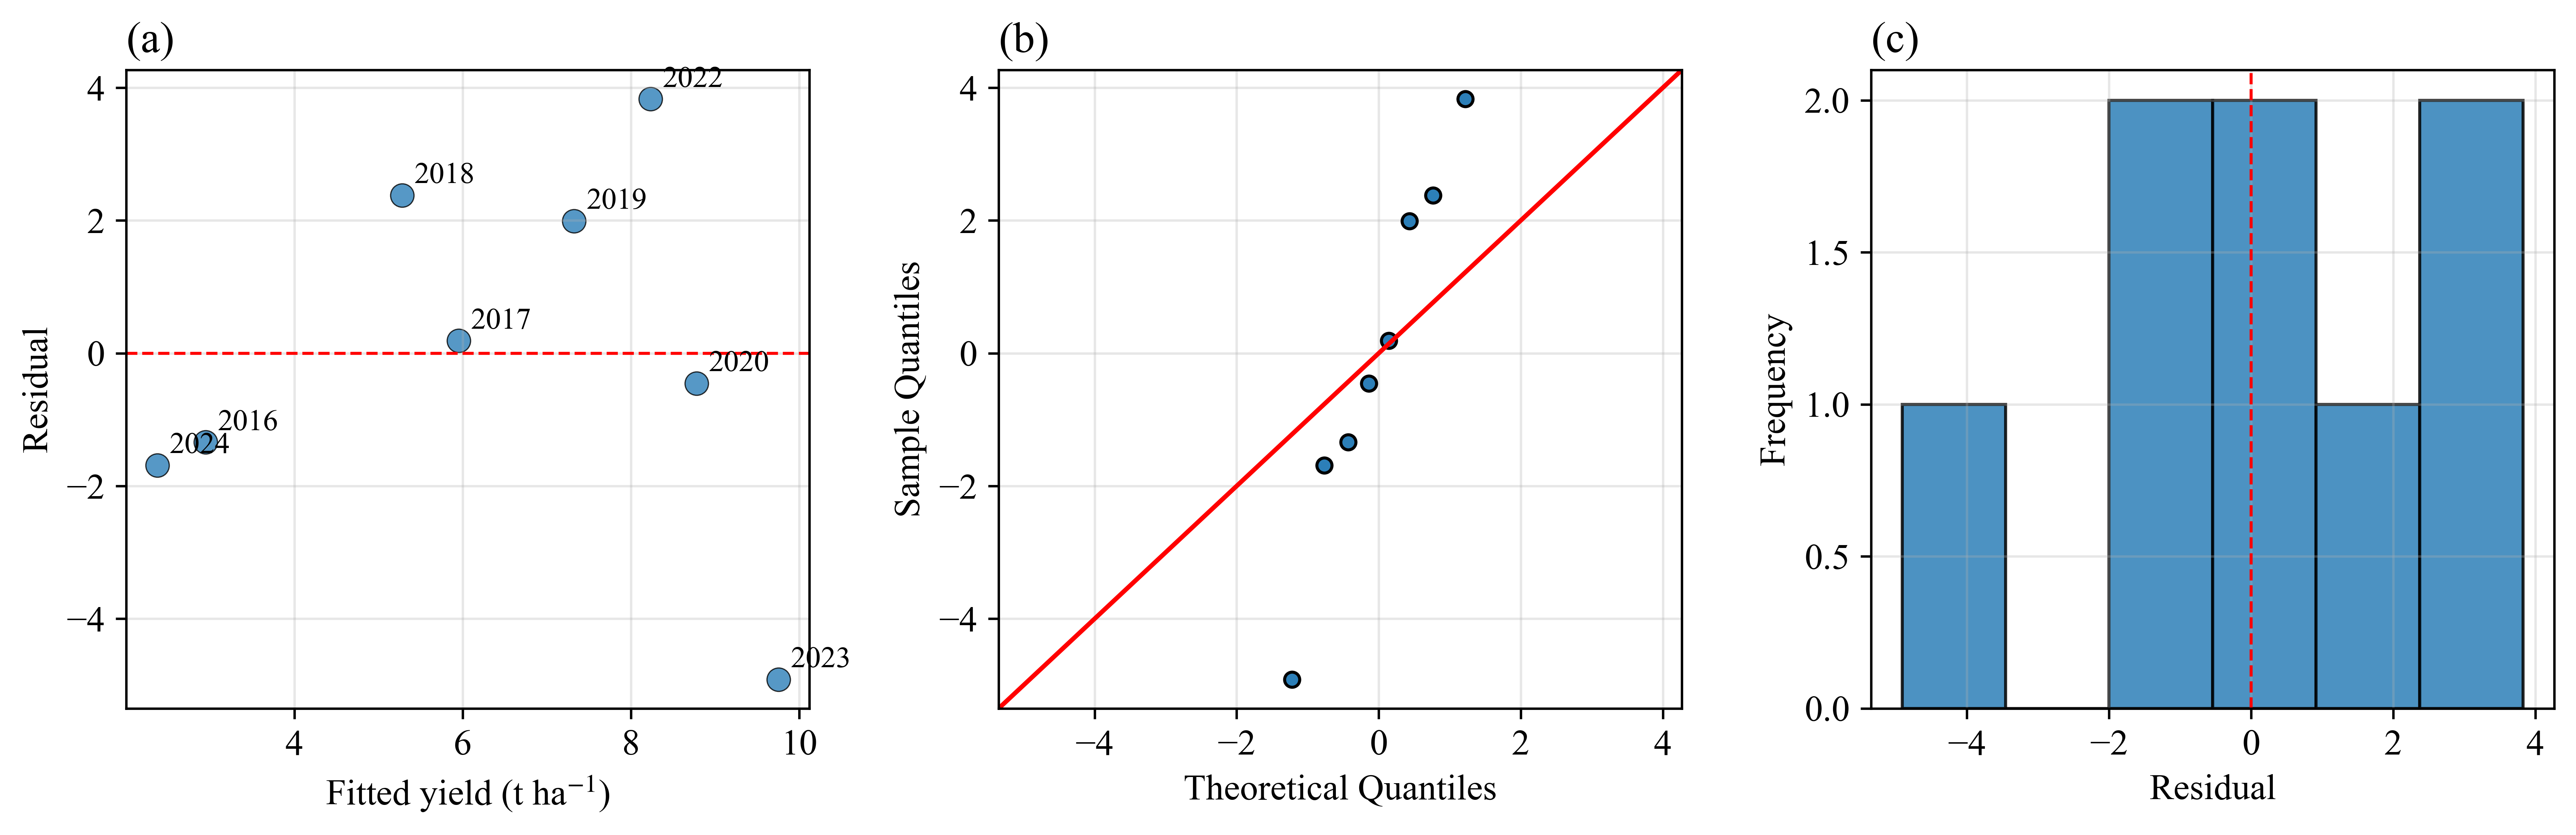
\includegraphics[width=\textwidth]{FigureS5.png}
\caption{In-sample residual diagnostics for the primary log-OLS model on the
back-transformed raw-yield scale (t~ha$^{-1}$). (\textbf{a})~Residuals vs.\ fitted
yield, labelled by harvest year; (\textbf{b})~Normal Q--Q plot; (\textbf{c})~Histogram
of residuals. Residuals are approximately Gaussian and homoscedastic within the
limits of $n=8$; leverage and Cook's-distance diagnostics are discussed in
Section~4.5 of the main text.\label{fig:S5}}
\end{figure}

% -- Figure S6: VPD anomaly check --
\begin{figure}[H]
\centering
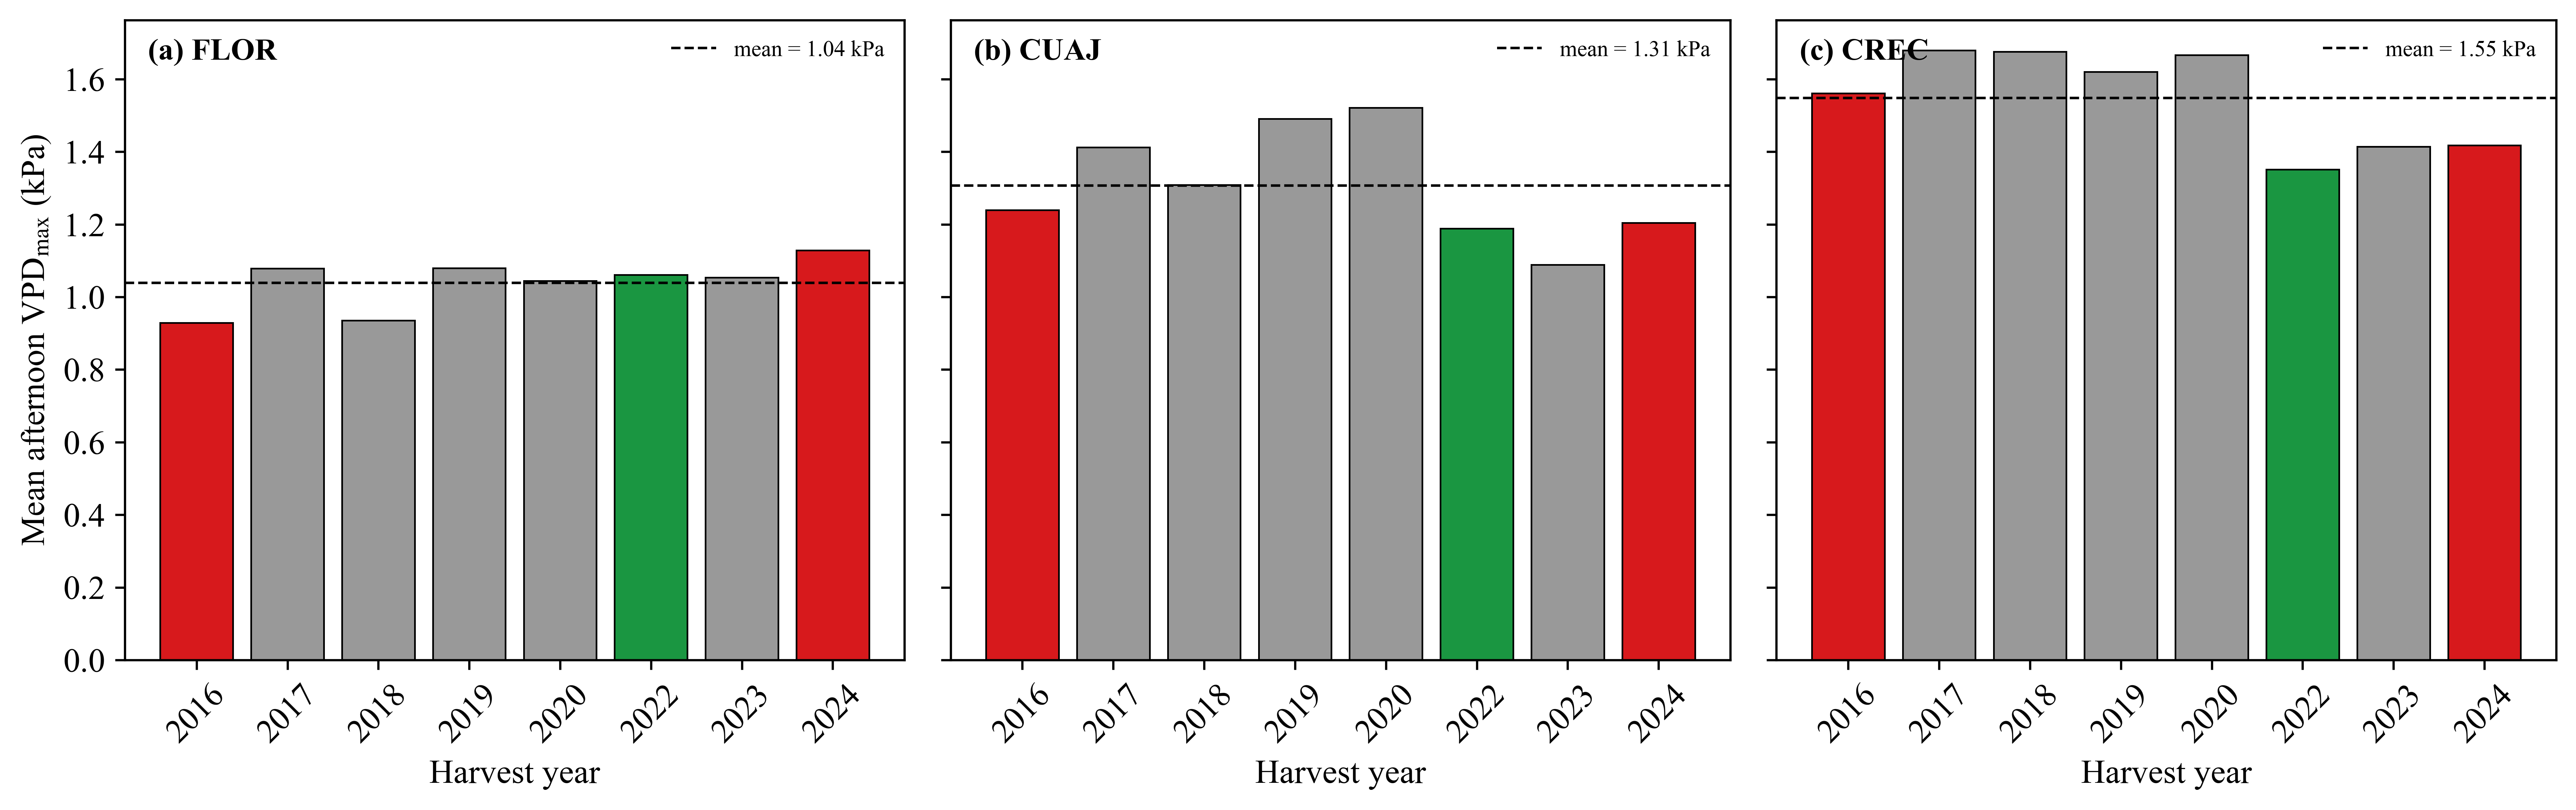
\includegraphics[width=\textwidth]{FigureS6.png}
\caption{Afternoon VPD$_{\max}$ proxy
($e_s(T_{\max})\,(1-\text{RH}_{\min}/100)$) averaged within the FLOR, CUAJ and
CREC phenology windows of each harvest year. Red: 2016 and 2024 failure years;
green: 2022 bumper year; dashed line: eight-year mean. The two failure years lie
within $\pm 10\,\%$ of the eight-year mean, ruling out atmospheric dryness as an
alternative driver of the observed yield collapses (Section~4.5 of the main
text).\label{fig:S6}}
\end{figure}

% -- Figure S7: Sentinel-2 mixed-pixel correction --
\begin{figure}[H]
\centering
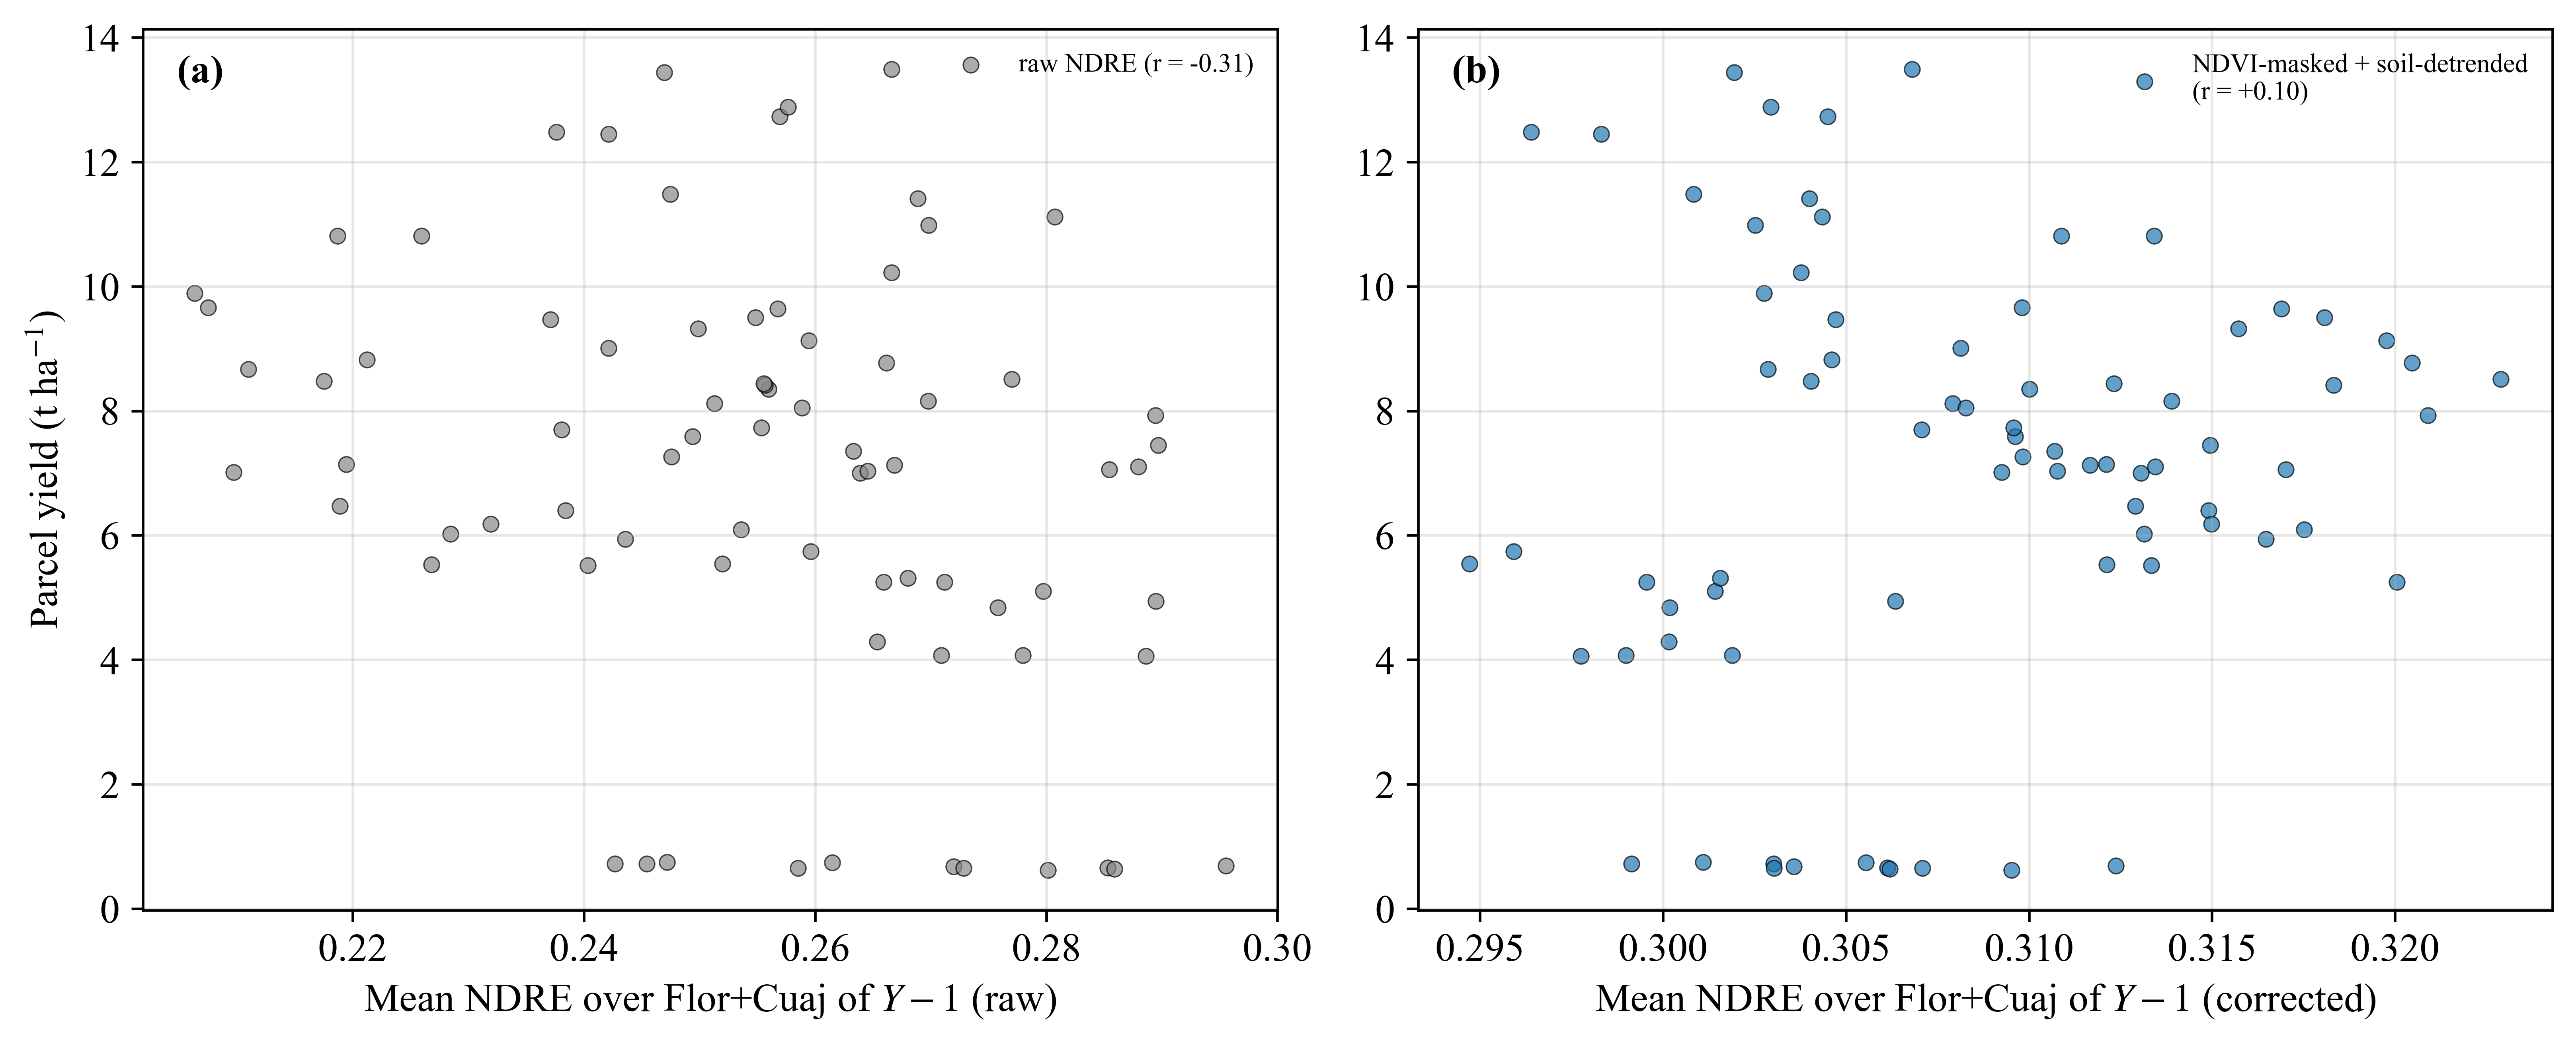
\includegraphics[width=\textwidth]{FigureS7.png}
\caption{Mixed-pixel mitigation for Sentinel-2 NDRE over the open-canopy
La~Yarada parcels ($n=77$ parcel-years). (\textbf{a})~Raw parcel-mean NDRE
composited over Flor+Cuaj of $Y-1$ vs.\ parcel-level annual yield.
(\textbf{b})~After an NDVI~$>0.25$ bare-soil mask and first-order linear
soil-detrending referenced to the canopy endmember NDVI$_{\text{pure}}=0.42$.
The pooled Pearson correlation rises from $r=-0.31$ (raw) to $r=+0.10$
(corrected), motivating the relegation of NDRE to a parcel-level descriptive
role (Section~3.6 of the main text).\label{fig:S7}}
\end{figure}

% -- Figure S8: Bayesian posterior of the chill slope --
\begin{figure}[H]
\centering
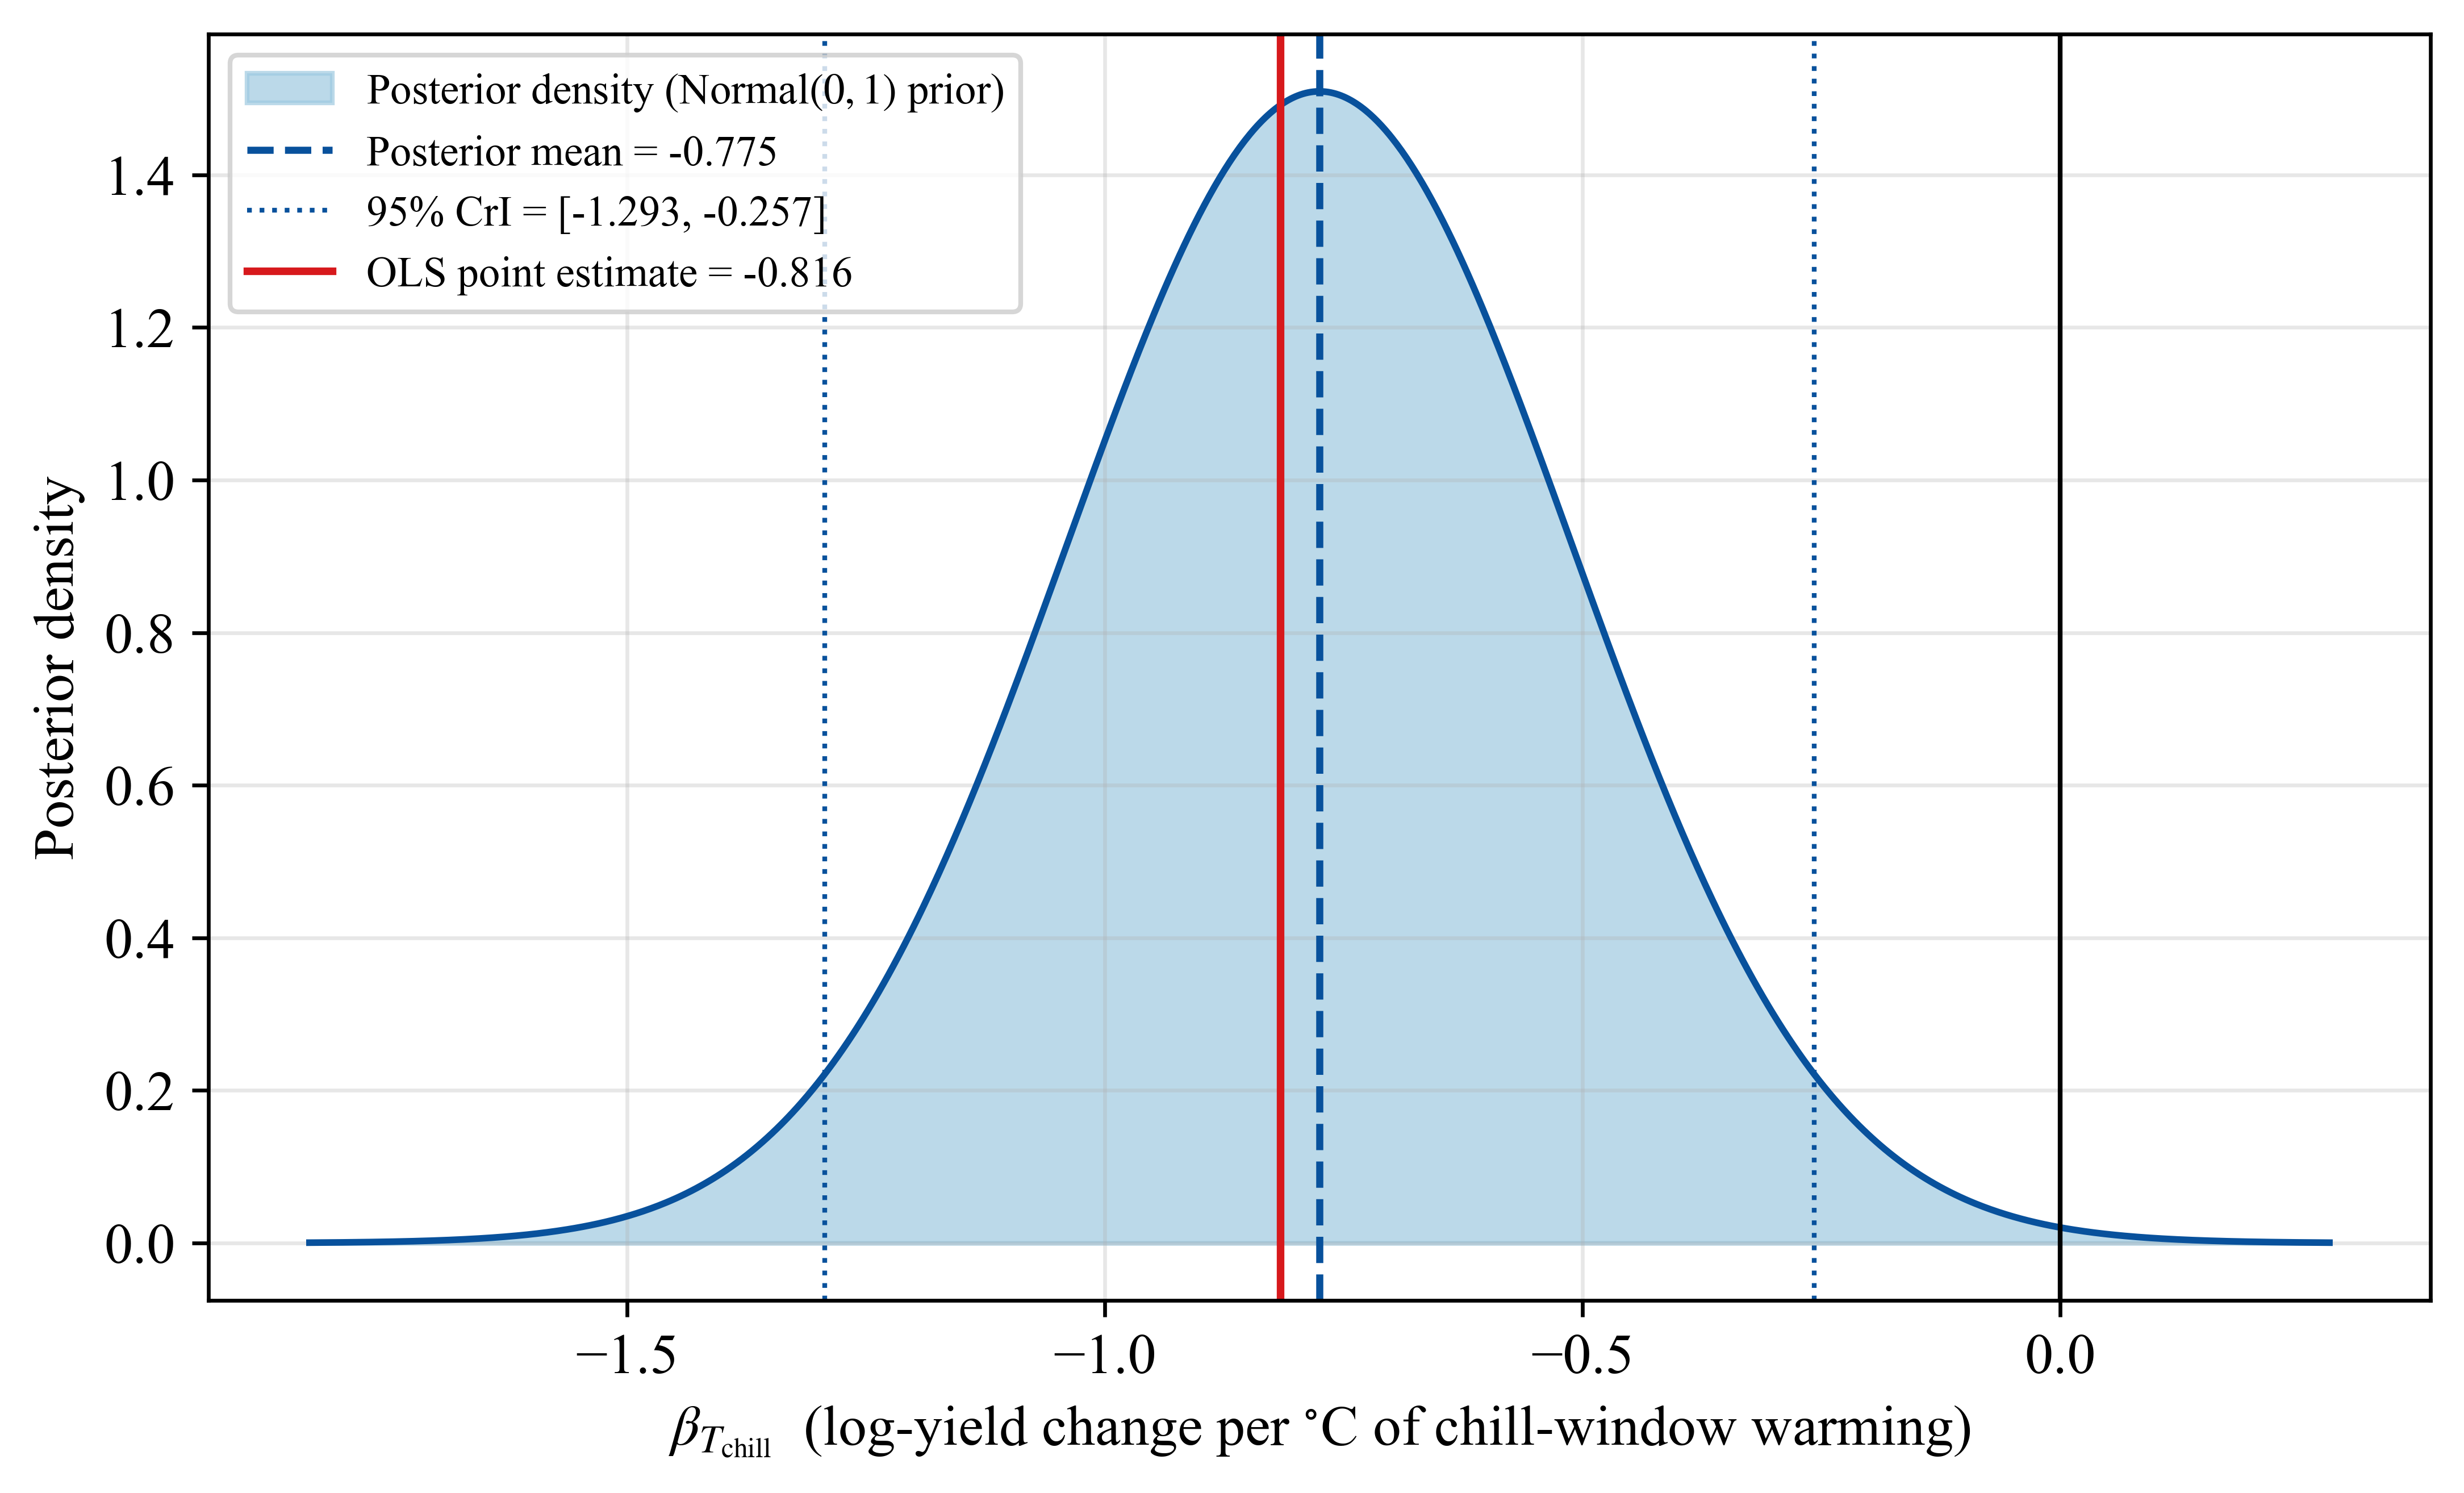
\includegraphics[width=0.85\textwidth]{FigureS8.png}
\caption{Closed-form Gaussian posterior of the chill slope
$\beta_{T_{\text{chill}}}$ (natural scale) under a weakly-informative
Normal$(0, 1)$ prior on the standardised coefficient. Posterior mean $-0.775$,
95\,\% CrI $[-1.293,\,-0.257]$; OLS point estimate $-0.816$ (red) is
indistinguishable from the posterior mean. The posterior mass lies entirely
below zero (Savage--Dickey BF$_{10}=15.9$), corroborating the frequentist
evidence (Section~3.3 of the main text).\label{fig:S8}}
\end{figure}

\FloatBarrier
\section*{Supplementary Tables}

% -- Table S1: Robustness summary --
% Table S1 — Robustness summary across alternative model specifications and LOYO variants
% Values taken directly from robustness_summary.csv (primary model, 07_final_primary_log.py;
% alt specs, 06_robustness_and_loyo_variants.py), oni_robustness.txt and alternance_sensitivity.txt.
\begin{table}[H]
\caption{Robustness summary of the primary attribution model across alternative
predictor pairs and cross-validation strategies. Metrics on the raw t~ha$^{-1}$
scale except \textit{loyo\_log} rows (log-space). Variants: \textit{in\_sample}
= full-calibration fit; \textit{loyo\_raw} = unbounded raw LOYO; \textit{loyo\_clipped}
= raw LOYO clipped to $[0,\,1.1\cdot y_{\max}]$; \textit{loyo\_log} = log-link LOYO;
\textit{loyo\_interior} = LOYO restricted to interior years (excluding the 2016 and
2024 warm-tail folds).\label{tab:robust_full}}
\centering
\footnotesize
\begin{tabular}{llccccc}
\toprule
\textbf{Variant} & \textbf{Stage} & \textbf{$n$} & \textbf{$R^{2}$} & \textbf{RMSE} & \textbf{MAE} & \textbf{Bias} \\
\midrule
\multicolumn{7}{l}{\textit{Primary: $T_{\text{chill}}$ + $T_{\text{CREC}}$}} \\
 & in\_sample      & 8 & $+0.108$ & $3.41$ & $2.54$ & $-0.40$ \\
 & loyo\_raw       & 8 & $\mathbf{-1.694}$ & $\mathbf{5.92}$ & $\mathbf{4.26}$ & $+0.31$ \\
 & loyo\_clipped   & 8 & $-0.756$ & $4.78$ & $3.69$ & $-0.26$ \\
 & loyo\_log       & 8 & $-0.071$ & $0.79$ & $0.65$ & $+0.08$ \\
 & loyo\_interior  & 4 & $+0.218$ & $2.67$ & $2.38$ & $-0.96$ \\
\midrule
\multicolumn{7}{l}{\textit{$T_{\text{chill}}$ only}} \\
 & in\_sample      & 8 & $+0.104$ & $3.41$ & $2.70$ & $-0.40$ \\
 & loyo\_raw       & 8 & $-1.452$ & $5.65$ & $4.00$ & $+0.47$ \\
 & loyo\_clipped   & 8 & $-0.290$ & $4.10$ & $3.32$ & $-0.21$ \\
 & loyo\_log       & 8 & $+0.199$ & $0.69$ & $0.58$ & $+0.09$ \\
 & loyo\_interior  & 5 & $+0.079$ & $2.60$ & $2.22$ & $-1.43$ \\
\midrule
\multicolumn{7}{l}{\textit{CP + $T_{\text{CREC}}$}} \\
 & in\_sample      & 8 & $-0.174$ & $3.91$ & $3.68$ & $-1.17$ \\
 & loyo\_raw       & 8 & $-15.608$ & $14.70$ & $10.11$ & $+3.87$ \\
\midrule
\multicolumn{7}{l}{\textit{CH$_{12}$ + $T_{\text{CREC}}$}} \\
 & in\_sample      & 8 & $-0.175$ & $3.91$ & $3.55$ & $-1.00$ \\
 & loyo\_raw       & 8 & $-8.648$ & $11.20$ & $8.25$ & $+2.44$ \\
\midrule
\multicolumn{7}{l}{\textit{$T_{\text{chill}}$ + $T_{\max,\text{FLOR}}$}} \\
 & in\_sample      & 8 & $+0.230$ & $3.16$ & $2.55$ & $-0.35$ \\
 & loyo\_raw       & 8 & $-1.139$ & $5.27$ & $4.12$ & $+0.24$ \\
\midrule
\multicolumn{7}{l}{\textit{RF (5 features)}} \\
 & loyo\_raw       & 8 & $-0.040$ & $3.68$ & $3.23$ & $+0.41$ \\
\midrule
\multicolumn{7}{l}{\textit{ONI$_{\text{May--Aug},t-1}$ + $T_{\text{CREC}}$ (ENSO robustness)}} \\
 & in\_sample      & 8 & $-0.080$ & $3.75$ & $3.19$ & --- \\
 & loyo\_raw       & 8 & $-3.562$ & $7.70$ & $5.97$ & --- \\
\midrule
\multicolumn{7}{l}{\textit{$T_{\text{chill}}$ + $T_{\text{CREC}}$ + share\_ON (alternance sensitivity)}} \\
 & in\_sample ($\beta_{T_{\text{chill}}}=-0.601$, $p=0.031$) & 8 & $+0.893$ & --- & --- & --- \\
\bottomrule
\end{tabular}
\end{table}


\FloatBarrier

% -- Table S2: Year-level Pearson correlations --
% Table S2 — Year-level Pearson correlations between yield and candidate predictors
% VALUES VERIFIED against year_level_correlations.csv (source of truth)
\begin{table}[H]
\caption{Year-level Pearson correlations between mean olive yield and candidate
climate predictors ($n=8$ years). $T_{\text{chill},t-1}$ ($r=-0.697$) is the
strongest single predictor; $T_{\text{CREC},t}$ was selected as the heat-side
predictor for its low collinearity with $T_{\text{chill},t-1}$ ($r=0.409$,
VIF\,$<2$) and its clean physiological decomposition. Threshold-based chill
counts (CP, CH$_{12}$) are weaker because they saturate at zero in the warm tail.\label{tab:year_corr}}
\centering
\small
\begin{tabular}{lcc}
\toprule
\textbf{Predictor} & \textbf{Pearson $r$ vs yield} & \textbf{Note} \\
\midrule
$T_{\text{chill},t-1}$ (May--Aug, $^\circ$C)     & $\mathbf{-0.697}$ & primary (chill side) \\
$T_{\max,\text{FLOR}}$ ($^\circ$C)               & $-0.492$ & flowering $T_{\max}$ \\
CH$_{12,t-1}$ (h)                                & $+0.404$ & threshold chill, h$<12\,^\circ$C \\
$T_{\text{mean},\text{FLOR}}$ ($^\circ$C)        & $-0.381$ & flowering window \\
$T_{\max,\text{CREC}}$ ($^\circ$C)               & $-0.375$ & fruit growth $T_{\max}$ \\
$T_{\text{CREC},t}$ (Jan--Mar, $^\circ$C)        & $\mathbf{-0.313}$ & primary (heat side) \\
CP$_{t-1}$ (Dynamic Model)                       & $+0.307$ & saturated at 0 in 5/8 years \\
ET$_{0,\text{CREC}}$ (mm)                        & $-0.178$ & FAO~56 reference ET, fruit growth \\
\midrule
\multicolumn{3}{l}{\textit{Cross-correlation $T_{\text{chill},t-1}\times T_{\text{CREC},t}=+0.409$ (moderate; VIF\,$<2$)}} \\
\bottomrule
\end{tabular}
\end{table}


\FloatBarrier

% -- Table S3: CMIP6 warming envelope --
% Table S3 — CMIP6 ensemble warming envelope used for the delta-method projections
\begin{table}[H]
\caption{CMIP6 warming envelope used for the delta-method projections: ensemble
central estimates and 5--95\,\% inter-model spread from the IPCC AR6 WGI Atlas,
region South-Western South America (SWS), relative to the 1995--2014 baseline.
Horizons are restricted to 2031--2050 and 2051--2070; the SSP5-8.5 2071--2100
ensemble median ($+4\,^{\circ}$C) is omitted as a 3$\times$ extrapolation beyond
the warmest observed chill year ($\Delta T_{\text{winter}}\approx +1.48\,^{\circ}$C).\label{tab:delta_envelope}}
\centering
\small
\begin{tabular}{llcccccc}
\toprule
\textbf{Scenario} & \textbf{Period} & \multicolumn{3}{c}{\textbf{$\Delta T_{\text{winter}}$ ($^\circ$C)}} & \multicolumn{3}{c}{\textbf{$\Delta T_{\text{summer}}$ ($^\circ$C)}} \\
\cmidrule(lr){3-5}\cmidrule(lr){6-8}
                  &                 & 5\,\% & median & 95\,\% & 5\,\% & median & 95\,\% \\
\midrule
SSP1-2.6 & 2031--2050 & 0.5 & 0.9 & 1.4 & 0.5 & 0.9 & 1.4 \\
SSP1-2.6 & 2051--2070 & 0.6 & 1.0 & 1.6 & 0.6 & 1.0 & 1.6 \\
\midrule
SSP2-4.5 & 2031--2050 & 0.6 & 1.1 & 1.6 & 0.6 & 1.1 & 1.6 \\
SSP2-4.5 & 2051--2070 & 1.0 & 1.6 & 2.3 & 1.0 & 1.6 & 2.2 \\
\midrule
SSP5-8.5 & 2031--2050 & 0.9 & 1.4 & 2.0 & 0.8 & 1.4 & 2.0 \\
SSP5-8.5 & 2051--2070 & 1.6 & 2.4 & 3.3 & 1.6 & 2.4 & 3.2 \\
\bottomrule
\end{tabular}
\end{table}


\FloatBarrier

% -- Table S4: Phenology windows --
% Table S4 — Phenology windows used for the climate aggregates
\begin{table}[H]
\caption{Phenology windows used to compute the climate and Sentinel-2 aggregates.
The chill window (Reposo+BROT, 1~May--31~Aug of $Y-1$) is the canonical
austral-winter chill window; floral induction (FLOR, CUAJ) occurs in $Y-1$;
fruit growth (CREC) and maturation (ENV) occur in $Y$.\label{tab:pheno_windows}}
\centering
\small
\begin{tabular}{llll}
\toprule
\textbf{Window} & \textbf{Start} & \textbf{End} & \textbf{Calendar year} \\
\midrule
Reposo + BROT (chill window) & 1 May  & 31 Aug & $Y-1$ \\
BROT (budburst)               & 15 Aug & 30 Sep & $Y-1$ \\
FLOR (flowering)              & 1 Oct  & 15 Nov & $Y-1$ \\
CUAJ (fruit set)              & 16 Nov & 31 Dec & $Y-1$ \\
CREC (fruit growth)           & 1 Jan  & 15 Mar & $Y$   \\
ENV (on-tree maturation)      & 16 Mar & 30 Apr & $Y$   \\
\bottomrule
\end{tabular}
\end{table}


\FloatBarrier

% -- Table S5: VPD aggregates and yield correlations --
% Table S5 — VPD aggregates and yield correlations
\begin{adjustwidth}{-\extralength}{0cm}
\begin{table}[H]
\caption{Vapour-pressure deficit (VPD, FAO~56) over the FLOR, CUAJ and CREC
phenology windows for each calibration year, plus year-level Pearson
correlations between VPD aggregates and observed yield ($n=8$). VPD$_{\text{m}}$
= within-window mean of daily mean VPD; VPD$_{\max,\text{m}}$ = within-window
mean of the daily afternoon proxy $e_s(T_{\max})\,(1-\text{RH}_{\min}/100)$;
VPD$_{\max,p95}$ = 95th percentile of the same proxy. 2016 and 2024 failure
years (bold) are not VPD-anomalous relative to the 2022 bumper year (italic);
yield--VPD correlations are weak ($|r|<0.36$ for the mean and afternoon-mean
metrics).\label{tab:vpd}}
\centering
\footnotesize
\setlength{\tabcolsep}{4pt}
\resizebox{\textwidth}{!}{%
\begin{tabular}{lccccccccc}
\toprule
& \multicolumn{3}{c}{\textbf{FLOR}} & \multicolumn{3}{c}{\textbf{CUAJ}} & \multicolumn{3}{c}{\textbf{CREC}} \\
\cmidrule(lr){2-4}\cmidrule(lr){5-7}\cmidrule(lr){8-10}
\textbf{Year} & VPD$_{\text{m}}$ & VPD$_{\max,\text{m}}$ & VPD$_{\max,p95}$ & VPD$_{\text{m}}$ & VPD$_{\max,\text{m}}$ & VPD$_{\max,p95}$ & VPD$_{\text{m}}$ & VPD$_{\max,\text{m}}$ & VPD$_{\max,p95}$ \\
& (kPa) & (kPa) & (kPa) & (kPa) & (kPa) & (kPa) & (kPa) & (kPa) & (kPa) \\
\midrule
\textbf{2016} & 0.479 & 0.929 & 1.131 & 0.643 & 1.240 & 1.413 & 0.783 & 1.561 & 1.851 \\
2017 & 0.581 & 1.079 & 1.238 & 0.637 & 1.412 & 1.662 & 0.845 & 1.679 & 2.130 \\
2018 & 0.486 & 0.935 & 1.095 & 0.615 & 1.309 & 1.638 & 0.823 & 1.676 & 2.013 \\
2019 & 0.549 & 1.079 & 1.290 & 0.724 & 1.491 & 1.761 & 0.752 & 1.620 & 1.963 \\
2020 & 0.448 & 1.044 & 1.593 & 0.649 & 1.521 & 1.879 & 0.705 & 1.667 & 2.205 \\
\textit{2022} & \textit{0.448} & \textit{1.061} & \textit{1.775} & \textit{0.525} & \textit{1.188} & \textit{1.903} & \textit{0.644} & \textit{1.351} & \textit{1.771} \\
2023 & 0.474 & 1.054 & 1.596 & 0.471 & 1.089 & 1.678 & 0.645 & 1.414 & 1.992 \\
\textbf{2024} & 0.491 & 1.128 & 1.586 & 0.547 & 1.204 & 1.679 & 0.642 & 1.418 & 1.898 \\
\midrule
\textbf{Mean} & 0.495 & 1.039 & 1.413 & 0.601 & 1.307 & 1.702 & 0.730 & 1.553 & 1.978 \\
\midrule
$r$ vs.\ yield & $-0.08$ & $+0.05$ & $+0.26$ & $+0.15$ & $+0.36$ & $+0.76$ & $-0.00$ & $+0.09$ & $+0.07$ \\
\bottomrule
\end{tabular}%
}
\end{table}
\end{adjustwidth}


\FloatBarrier

% -- Table S6: Leave-out sensitivity --
% Table S6 — Leave-out sensitivity of the primary log-OLS model
% Values taken verbatim from sensitivity_leave_out.csv (script 07b_sensitivity_leave_out.py)
\begin{table}[H]
\caption{Leave-out sensitivity of the primary log-OLS model
$\log(y+0.5)\sim T_{\text{chill},t-1}+T_{\text{CREC},t}$, refit on the full
eight-year sample, with 2024 removed, and with both warm-tail years
(2016, 2024) removed. Removing 2024 alone halves the chill slope
($p=0.37$); removing both warm-tail anchors collapses the chill-window
range to $\sim$1.5\,$^{\circ}$C and flips the fitted slope
($+0.32$, $p=0.44$), quantifying how much attribution skill is carried
by the two extreme years.\label{tab:sens_leave_out}}
\centering
\footnotesize
\begin{tabular}{lccccccc}
\toprule
\textbf{Variant} & \textbf{$n$} & \textbf{$\beta_{T_{\text{chill}}}$ (SE)} & \textbf{$p_{\text{chill}}$} & \textbf{$\beta_{T_{\text{CREC}}}$} & \textbf{$p_{\text{CREC}}$} & \textbf{$R^{2}_{\log}$} & \textbf{$R^{2}_{\text{raw}}$} \\
\midrule
Full (2016--2024, ex 2021)         & 8 & $-0.816\,(0.272)$ & $0.0299$ & $+0.089$ & $0.529$ & $0.653$ & $0.108$ \\
Leave 2024                          & 7 & $-0.433\,(0.428)$ & $0.3681$ & $-0.033$ & $0.853$ & $0.396$ & $0.091$ \\
Leave \{2016, 2024\}                & 6 & $+0.322\,(0.360)$ & $0.4374$ & $-0.107$ & $0.368$ & $0.284$ & $0.341$ \\
\bottomrule
\end{tabular}
\end{table}


\FloatBarrier

% -- Table S7: Offset sensitivity --
% Table S7 — Sensitivity to the offset constant c in log(y+c)
% Values taken verbatim from sensitivity_offset.csv (script 07b_sensitivity_leave_out.py)
\begin{table}[H]
\caption{Sensitivity of the primary log-OLS model
$\log(y+c)\sim T_{\text{chill},t-1}+T_{\text{CREC},t}$ to the offset
constant $c$, using the full eight-year sample. The chill slope varies
monotonically with $c$ (from $-0.961$ at $c=0.1$ to $-0.697$ at $c=1.0$)
but remains significant throughout ($p\leq 0.035$); sign and significance
of the chill effect are preserved across the practical range of
offsets.\label{tab:sens_offset}}
\centering
\footnotesize
\begin{tabular}{cccccccc}
\toprule
\textbf{$c$} & \textbf{$n$} & \textbf{$\beta_{T_{\text{chill}}}$ (SE)} & \textbf{$p_{\text{chill}}$} & \textbf{$\beta_{T_{\text{CREC}}}$} & \textbf{$R^{2}_{\log}$} & \textbf{$R^{2}_{\text{raw}}$} & \textbf{RMSE$_{\text{raw}}$} \\
\midrule
$0.10$ & 8 & $-0.961\,(0.306)$ & $0.0255$ & $+0.118$ & $0.671$ & $0.011$ & $3.59$ \\
$0.25$ & 8 & $-0.899\,(0.291)$ & $0.0272$ & $+0.105$ & $0.663$ & $0.053$ & $3.51$ \\
$0.50$ & 8 & $-0.816\,(0.272)$ & $0.0299$ & $+0.089$ & $0.653$ & $0.108$ & $3.41$ \\
$0.75$ & 8 & $-0.751\,(0.256)$ & $0.0324$ & $+0.077$ & $0.643$ & $0.149$ & $3.33$ \\
$1.00$ & 8 & $-0.697\,(0.242)$ & $0.0347$ & $+0.067$ & $0.635$ & $0.181$ & $3.26$ \\
\bottomrule
\end{tabular}
\end{table}


\FloatBarrier

% -- Table S8: Annual climate summary --
% Table S8 — Annual climate summary for the calibration sample
% Values taken verbatim from year_level_dataset_extended.csv (yield & all climate predictors)
\begin{adjustwidth}{-\extralength}{0cm}
\begin{table}[H]
\caption{Annual climate summary for the eight-year calibration sample
(2016--2024, ex 2021). For each harvest year $Y$: parcel-mean olive yield
with between-parcel SD ($n=11$ parcels), chill-window ($Y-1$) Dynamic-Model
Chill Portions (CP) and Chill Hours below $12\,^\circ$C (CH$_{12}$),
chill-window mean temperature $T_{\text{chill},t-1}$, flowering-window and
fruit-growth temperatures, fruit-growth ET$_0$ (FAO~56), and NOAA ONI
averaged over the chill window. El~Ni\~{n}o failure years (2016, 2024) in
bold; triple-La~Ni\~{n}a bumper year (2022) in italic.\label{tab:annual_summary}}
\centering
\footnotesize
\setlength{\tabcolsep}{3pt}
\resizebox{\textwidth}{!}{%
\begin{tabular}{cccccccccccc}
\toprule
\textbf{Year} & \textbf{Yield} & \textbf{SD} & \textbf{CP} & \textbf{CH$_{12}$} & \textbf{$T_{\text{chill}}$} & \textbf{$T_{\max,\text{FLOR}}$} & \textbf{$T_{\text{mean,FLOR}}$} & \textbf{$T_{\max,\text{CREC}}$} & \textbf{$T_{\text{CREC}}$} & \textbf{ET$_{0,\text{CREC}}$} & \textbf{ONI$_{\text{chill}}$} \\
$Y$ & (t\,ha$^{-1}$) & (t\,ha$^{-1}$) & (portions) & (h) & ($^\circ$C) & ($^\circ$C) & ($^\circ$C) & ($^\circ$C) & ($^\circ$C) & (mm) & ($^\circ$C) \\
\midrule
\textbf{2016} & \textbf{1.60} & 0.19 & 0.00 & 63  & \textbf{18.20} & 22.23 & 18.71 & 27.50 & 23.39 & 365.0 & $+1.44$ \\
2017          & 6.14          & 0.60 & 0.00 & 132 & 17.19          & 22.56 & 18.98 & 28.17 & 23.99 & 379.0 & $-0.08$ \\
2018          & 7.66          & 0.68 & 0.00 & 85  & 17.46          & 21.12 & 17.47 & 26.98 & 21.96 & 268.1 & $+0.23$ \\
2019          & 9.32          & 0.92 & 0.00 & 100 & 16.77          & 22.74 & 18.86 & 27.52 & 22.46 & 281.8 & $+0.09$ \\
2020          & 8.33          & 0.86 & 1.00 & 147 & 16.32          & 21.79 & 17.03 & 27.36 & 21.11 & 315.0 & $+0.42$ \\
\textit{2022} & \textit{12.06} & \textit{1.08} & \textit{3.03} & \textit{417} & \textit{16.56} & \textit{22.09} & \textit{15.95} & \textit{24.77} & \textit{18.66} & \textit{247.6} & \textit{$-0.37$} \\
2023          & 4.84          & 0.62 & 4.02 & 489 & 16.03          & 22.09 & 16.20 & 26.01 & 19.83 & 202.5 & $-0.83$ \\
\textbf{2024} & \textbf{0.68} & 0.04 & 0.00 & 30  & \textbf{18.45} & 23.81 & 17.92 & 26.84 & 20.56 & 254.8 & $+0.98$ \\
\midrule
\textbf{Mean} & 6.33          & ---  & 1.01 & 183 & 17.25          & 22.30 & 17.64 & 26.90 & 21.50 & 289.2 & $+0.11$ \\
\bottomrule
\end{tabular}%
}
\end{table}
\end{adjustwidth}


\FloatBarrier

%=================================================================
\end{document}
